\documentclass[12pt]{report}
% Definición de márgenes
\usepackage[a4paper,bindingoffset=2mm,left=25mm,right=25mm,top=30mm,bottom=30mm,footskip=5mm]{geometry}
% Idioma español
\usepackage{listingsutf8}
\usepackage[spanish]{babel}
\renewcommand\spanishtablename{Tabla}
% Para que se generen los acentos correctamente
\usepackage[utf8]{inputenc}
% Imagenes
\usepackage{graphicx}
\usepackage{float}
\usepackage{subfig}
\usepackage{rotating}
\usepackage{tikz}
% Mejoras para las listas
\usepackage{enumitem}
% Notacion cientifica para los numeros
\usepackage{siunitx}
% Referencias \ref
\usepackage{nameref}

% Codigo MATLAB
\usepackage{listings}
\usepackage{color} %red, green, blue, yellow, cyan, magenta, black, white
\definecolor{mygreen}{RGB}{28,172,0} % color values Red, Green, Blue
\definecolor{mylilas}{RGB}{170,55,241}
\definecolor{codebg}{RGB}{220,220,220}

% Subtitulos!
\usepackage{titling}
\newcommand{\subtitle}[1]{%
  \posttitle{%
    \par\end{center}
    \begin{center}\large#1\end{center}
    \vskip0.5em}%
}

% Headers y Footers
\usepackage{fancyhdr}
\pagestyle{fancy}
\lhead{UTN San Francisco}
\rhead{Anchino Leonardo -- Torti Andrés}
\cfoot{\thepage}

% Ecuaciones
\usepackage{amsmath,mathtools}
\usepackage{amssymb}
\usepackage{kantlipsum}
\usepackage[makeroom]{cancel}
\allowdisplaybreaks
% Paginas Horizontales
\usepackage{pdflscape}
% URLs y Referencias
\usepackage[hidelinks]{hyperref}

% Centrado vertical en tablas
\usepackage{array, booktabs}
\newcolumntype{M}[1]{>{\centering\arraybackslash}m{#1}}
\newcolumntype{L}[1]{>{\raggedright\let\newline\\\arraybackslash\hspace{0pt}}m{#1}}

% Simbolo de grados
\usepackage{textcomp}
\usepackage{gensymb}

\begin{document}
\author{Torti Andrés - Anchino Leonardo}
	
\begin{titlepage}
	\title{\Huge Diseño y construcción de fuente conmutada tipo Buck de 75W}
	\subtitle{Análisis en detalle del diseño y desarrollo de una fuente conmutada para presentarse como trabajo final en la Universidad Tecnológica Nacional de la ciudad de San Francisco, Córdoba}
	\date{21 de Diciembre de 2016}
	\maketitle
\end{titlepage}

\tableofcontents
\listoffigures
\newpage
	
\chapter{Introducción}
\section{Objetivos}
El objetivo de este proyecto fue construir una fuente conmutada de 75W que provea diversidad de tensiones de salida reguladas y controladas por medio de un sistema PID. Se hará uso de dos convertidores tipo Buck para las salidas principales y regulables de potencia, así como otros reguladores existentes en el mercado para proveer tensiones fijas y auxiliares. Todo el sistema será controlado por medio de un DSP que implementará el sistema de control PID. El proyecto tiene un fin meramente de investigación y representa un reto ya que el tema fuentes conmutadas no se desarrolla durante la carrera.

Se plantearon las siguientes especificaciones para la fuente:

\begin{table}[H]
	\centering
	\begin{tabular}{M{2cm}M{5cm}M{1cm}M{1cm}M{1cm}M{1cm}} \toprule
		Parámetro & Descripción & Min & Tip & Max & Unidad
		\\ \midrule
		$V_{in}$ & Tensión de entrada & 200 & 220 & 240 & VAC \\
		$V_{buck(1)}$ & Tensión de Buck 1 & 1 & - & 20 & V \\
		$I_{buck(1)}$ & Corriente de salida Buck 1 & 0 & - & 3 & A \\
		$V_{ripple(1)}$ & Tensión de ripple de Buck 1 & - & - & 10 & mV \\
		\multicolumn{6}{c}{ } \\
		$V_{buck(2)}$ & Tensión de Buck 2 & 1 & - & 20 & V \\
		$I_{buck(2)}$ & Corriente de salida Buck 2 & 0 & - & 3 & A \\
		$V_{ripple(2)}$ & Tensión de ripple de Buck 2 & - & - & 10 & mV \\
		\multicolumn{6}{c}{ } \\
		$V_{out(3)}$ & Tensión de salida 3 & 3.2 & 3.3 & 3.4 & V \\
		$I_{out(3)}$ & Corriente de salida 3 & 0 & - & 300 & mA \\
		$V_{out(4)}$ & Tensión de salida 4 & 4.9 & 5 & 5.1 & V \\
		$I_{out(4)}$ & Corriente de salida 4 & 0 & - & 1 & A \\
		\multicolumn{6}{c}{ } \\
		$\eta$ & Eficiencia estimada & \multicolumn{3}{c}{80} & \% \\
		\\ \bottomrule
	\end{tabular}
	\caption{Parámetros de la fuente}
\end{table}

\textbf{Es importante aclarar que los 75W de salida son compartidos entre todas las salidas, es decir, no podríamos sacar 20V a 3A en ambos Buck al mismo tiempo ya que estaríamos excediendo los 75W máximos. Lo mismo sucede con las salidas de +3.3V y +5V, los 75W son distribuidos entre las cuatro salidas.}

El siguiente diagrama en bloques representa la estructura general de la fuente, cada bloque será analizado en detalle en los capítulos posteriores:

\begin{figure}[H]
	\centering
	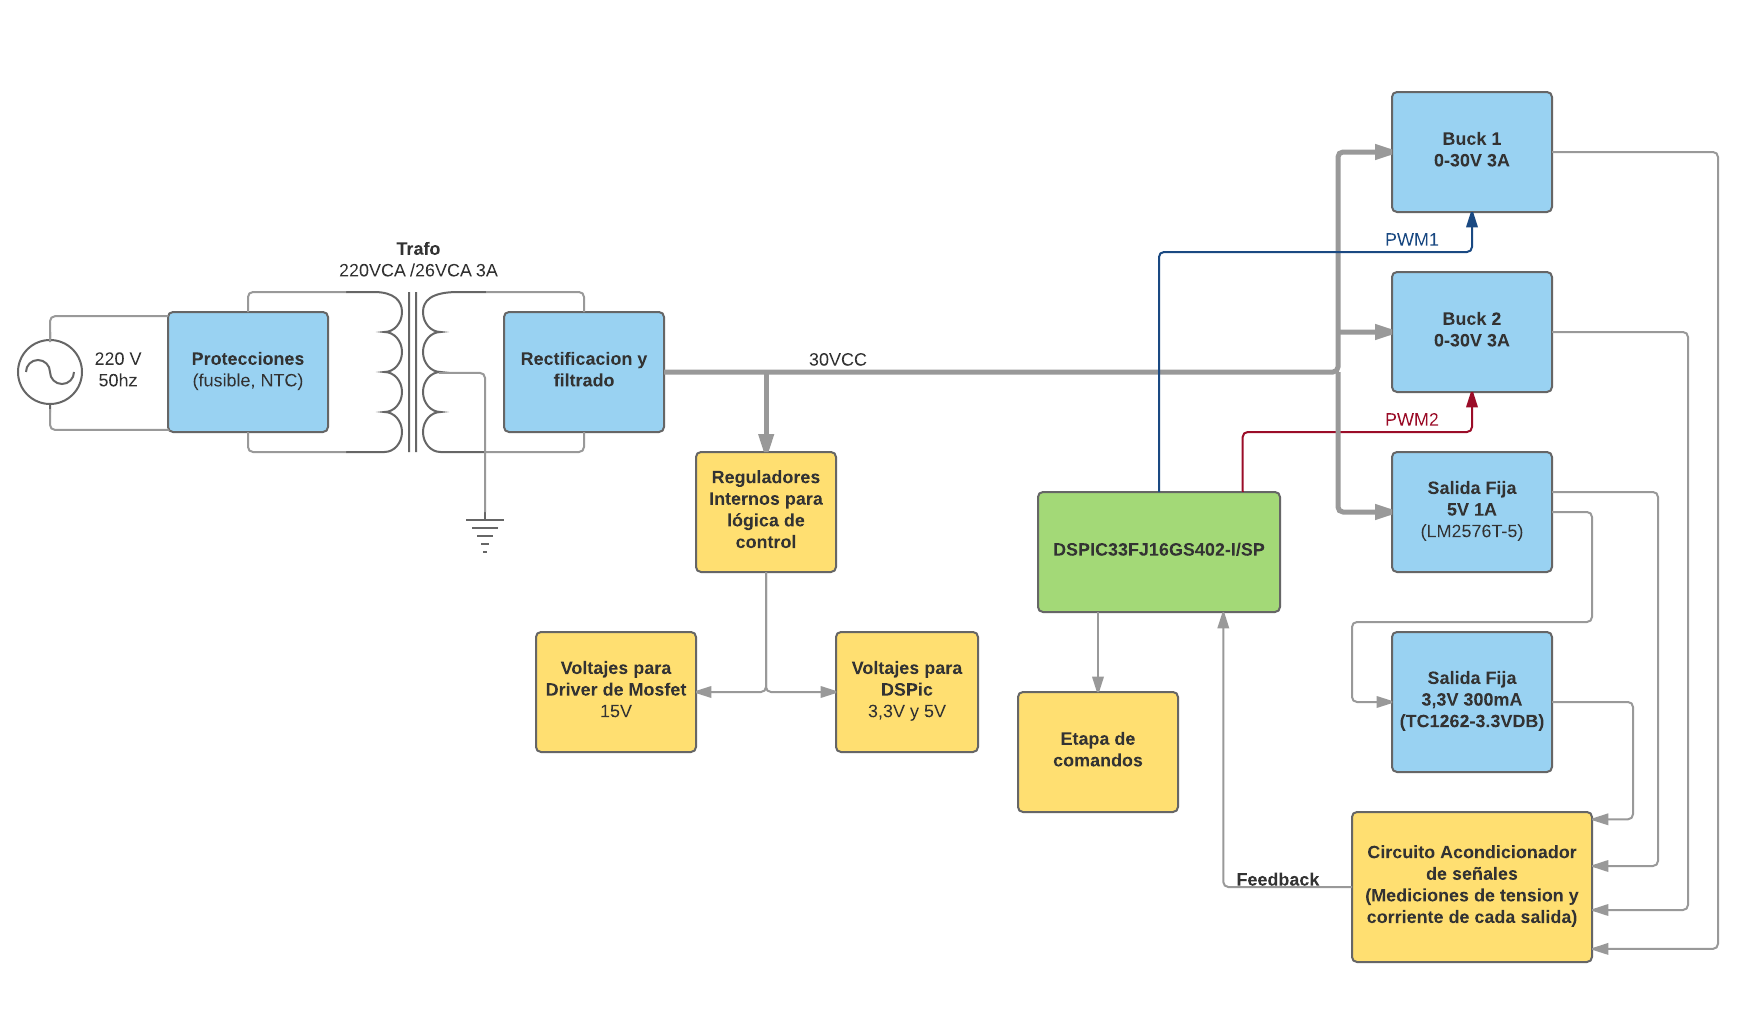
\includegraphics[width=\textwidth,height=\textheight,keepaspectratio]{diagrama_bloques}
	\caption{Diagrama en bloques del sistema}
\end{figure}

\section{Sistema de control PID}

Para poder lograr una tensión estable y regulada en la salida se debe implementar un lazo de realimentación, en nuestro caso, un sistema PID fue elegido debido a que el mismo nos permitirá no solo controlar de forma precisa la tensión de salida sino que también evitará transitorios que puedan ocurrir por ejemplo durante la conexión y desconexión de dispositivos a la fuente o cambios bruscos de corriente.

\begin{figure}[H]
	\centering
	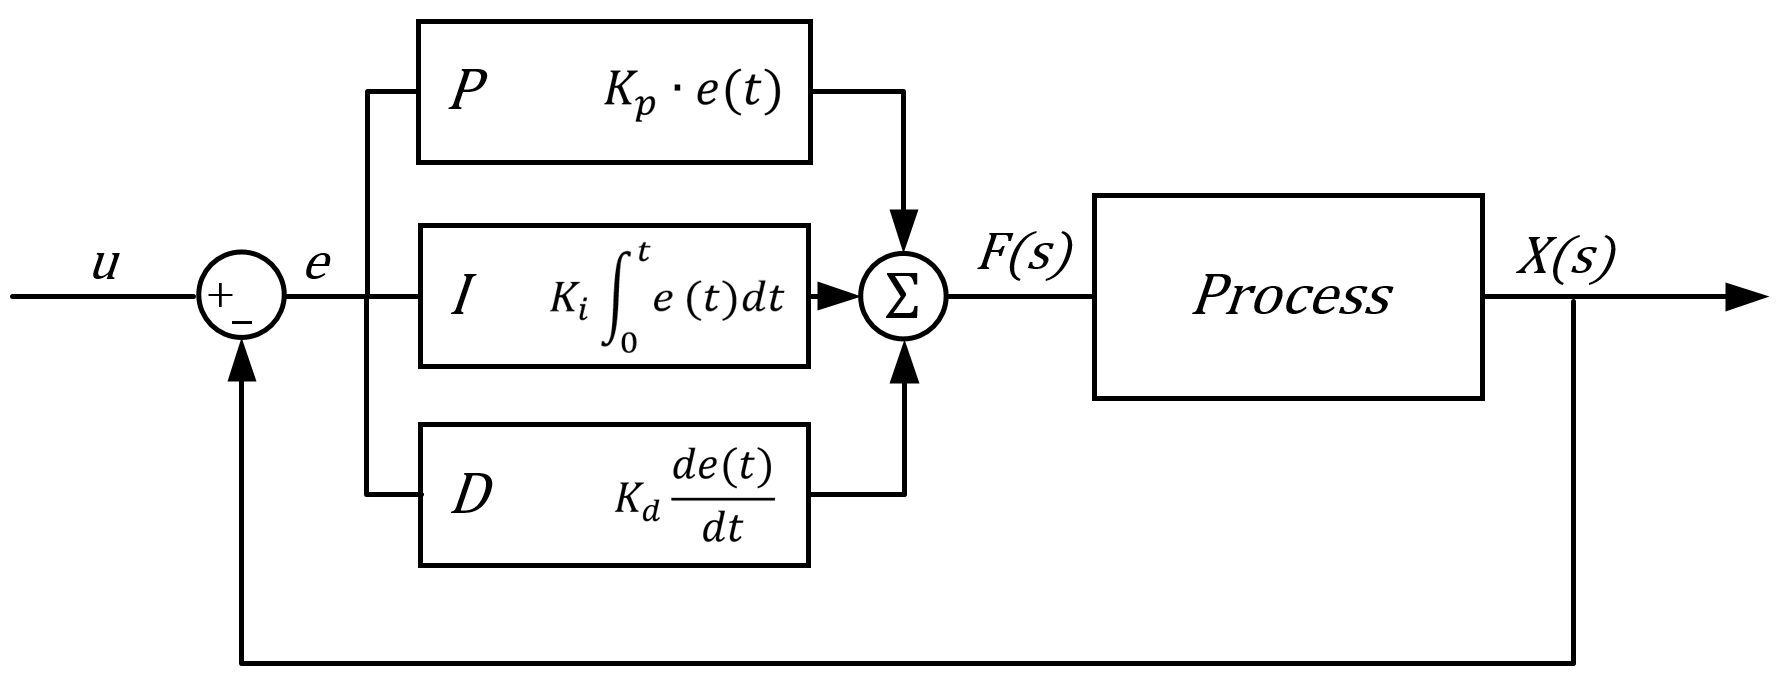
\includegraphics[width=\textwidth,height=\textheight,keepaspectratio]{closed_loop}
	\caption{Sistema de lazo cerrado}
\end{figure}

En el capítulo \textit{\nameref{chapter:pid}} desarrollaremos y explicaremos la función de transferencia del sistema de forma detallada y calcularemos los coeficientes del controlador PID con ayuda del software MATLAB\textregistered \ para así simular su comportamiento y compararlo con el circuito real implementado.

\chapter{Convertidores Buck}

\section{Principio de funcionamiento}

	La fuente posee dos salidas regulables e independientes de potencia que fueron implementadas con dos convertidores Buck idénticos. Cada \textit{Convertidor Buck} o \textit{Buck Converter} en Inglés tiene su entrada conectada a los +30V DC que provienen de la salida rectificada y filtrada del transformador y es el encargado de reducir la tensión que se le suministra para proveer un rango que varia entre 1V y 30V aproximadamente. 
	
	A continuación se presenta un diagrama simplificado de la topología Buck:
	
	\begin{figure}[H]
		\centering
		\includegraphics[width=\textwidth,height=\textheight,keepaspectratio]{buck_topology}
		\caption{Esquema simplificado de un convertidor tipo Buck}
	\end{figure}

	\begin{figure}[H]
		\centering
		\includegraphics[width=\textwidth,height=\textheight,keepaspectratio]{buck_currents}
		\caption{Diagrama de corrientes del convertidor Buck}
		\label{buck:currents}
	\end{figure}

	Como podemos observar existen dos estados durante la operación del Buck. El primero de ellos es cuando el interruptor se encuentra cerrado durante un tiempo $T_{on}$ como se observa en la figura \ref{buck:currents}, en este instante una tensión constante $\approx V_{in}$ es aplicada sobre el inductor por lo que la corriente comienza a aumentar de forma lineal y por consiguiente producirá una tensión inversa en respuesta al incremento de la corriente que es a su vez opuesta a la fuente, por lo tanto la tensión vista por la carga es menor a $V_{in}$.
	
	En el segundo estado cuando abrimos el interruptor durante el tiempo $T_{off}$, la energía almacenada en el inductor es la que produce la circulación de corriente que alimenta al circuito a través del diodo en paralelo.
	
	En la práctica, el interruptor es reemplazado en general por un MOSFET de baja $R_{ds(on)}$ y el tipo de diodo es en general de tipo Schottky debido a su alta velocidad de conmutación, baja caída de tensión y baja capacidad parásita. En nuestro caso se optó por un circuito ligeramente distinto en donde el diodo es reemplazado por otro transistor MOSFET en donde el principio de funcionamiento es idéntico pero se reducen las pérdidas producidas por el diodo. A este tipo de Buck se lo conoce como \textit{Convertidor Buck Sincrónico} o \textit{Synchronous Buck Converter}. El esquema del convertidor Buck final se muestra a continuación:

	\newpage
	\begin{landscape}
		\newpage
		\begin{figure}[p]
			\centering
			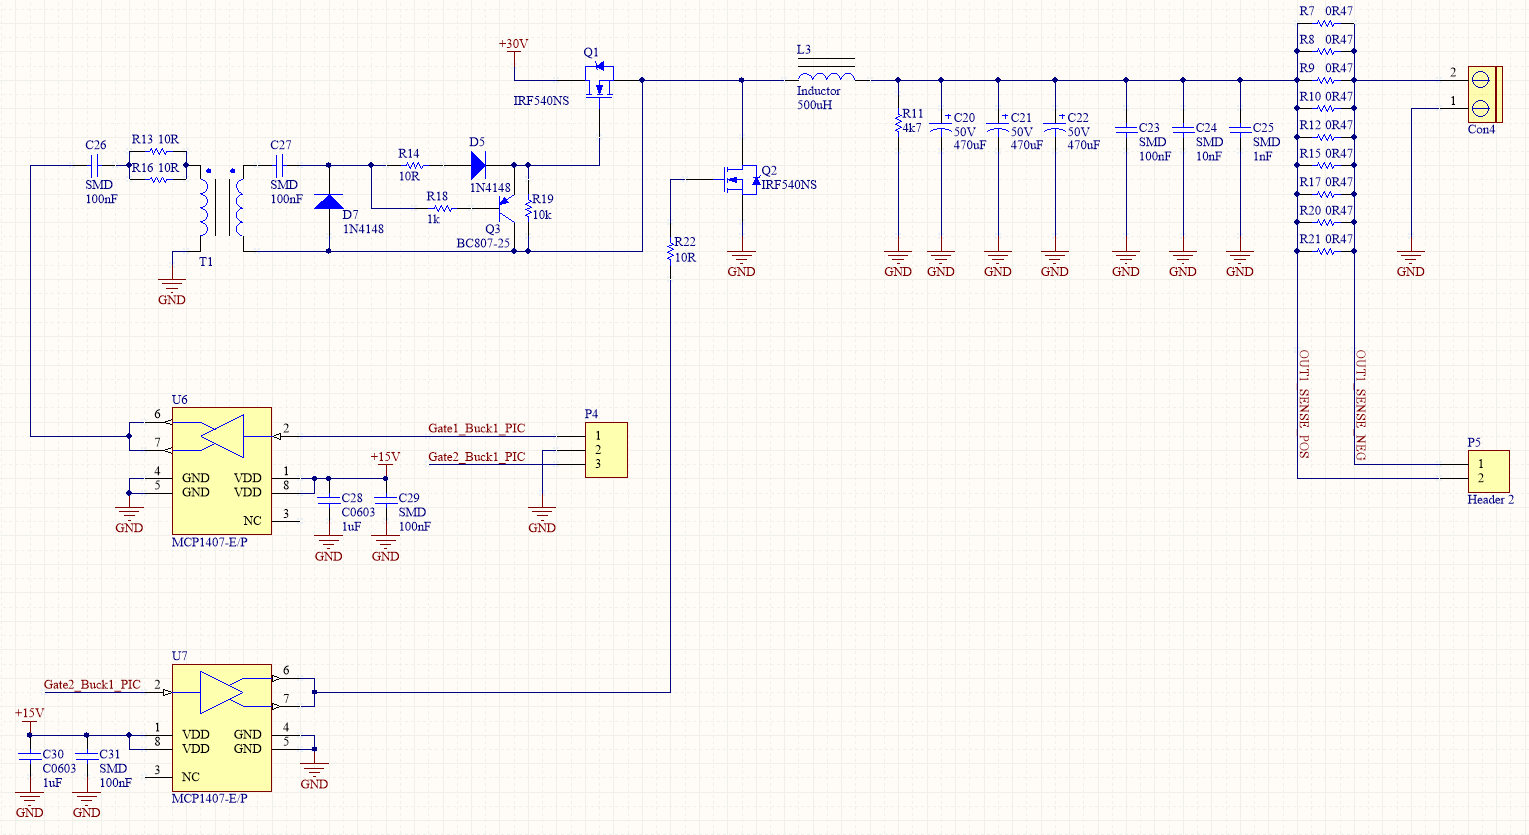
\includegraphics[width=\paperwidth,height=\paperheight,keepaspectratio]{buck_schematic}
			\caption{Esquema del Convertidor Buck Sincrónico}
		\end{figure}
	\end{landscape}

	Para los cálculos de la mayor parte de los componentes del convertidor se utilizó la nota de aplicación "\href{http://www.ti.com/lit/an/slva477b/slva477b.pdf}{Basic Calculation of a Buck Converter's Power Stage}" de Texas Instruments.
	
	Antes de realizar el cálculo de los componentes del convertidor presentamos los parámetros elegidos para su diseño:
	
	\begin{table}[H]
		\centering
		\begin{tabular}{M{2cm}M{5cm}M{1cm}M{1cm}M{1cm}M{1cm}} \toprule
			Parámetro & Descripción & Min & Tip & Max & Unidad
			\\ \midrule
			$V_{out}$ & Tensión de salida & 1 & - & 30 & V \\
			$I_{out}$ & Corriente de salida & 0 & - & 3 & A \\
			$V_{ripple}$ & Tensión de ripple pico a pico & - & - & 10 & mV \\
			$I_{ripple}$ & Corriente de ripple del inductor & \multicolumn{3}{c}{100} & mA \\
			$F_{sw}$ & Frecuencia de conmutación & \multicolumn{3}{c}{150} & KHz \\
			\bottomrule
		\end{tabular}
		\caption{Parámetros de la fuente}
	\end{table}
	
\section{Cálculo del inductor}
	
	El valor del inductor viene dado por la ecuación:
	
	\begin{equation}
		\begin{aligned}
		\qquad \qquad L_{min} [\mu H] &= \dfrac{V_{out} \cdot (V_{in} - V{out})}{\Delta I \cdot f_{sw} \cdot V_{in}} \cdot \num{10e6} \\
		& = \dfrac{15 \cdot (30 - 15)}{\num{100e-3} \cdot \num{150e3} \cdot 30} \cdot \num{10e6}\\
		& = 500 \mu H
		\end{aligned}
	\end{equation}
	
	Significa que necesitaremos un inductor de al menos $500\mu H$. Podemos ver que se eligió una tensión de salida de 15V para el cálculo cuando las especificaciones dicen que la misma varía entre 0 y 20V; esto es debido a que cuando la tensión de salida es variable se debe considerar el peor caso que es cuando $V_{out} = V_{in}/2$, en ese punto es donde se requiere el mayor valor de inductancia para mantener la corriente de ripple dentro de los límites establecidos.
	
	La elección de la corriente de ripple es una solución de compromiso, aumentar la misma nos permite utilizar valores de inductancia más pequeños pero degradando la regulación y produciendo un mayor estrés sobre el capacitor de salida que debe ser seleccionado para soporta la misma, así como un mayor ripple provocado por el ESR del capacitor, además, la corriente de salida mínima para no entrar en operación de modo discontinuo está directamente relacionada con la corriente de ripple siendo la relación $I_{out(min)} = I_{ripple}/2$ aunque cabe destacar que dicho efecto no se produce en los convertidor Buck Sincrónicos como en nuestro caso ya que al reemplazar el diodo por un MOSFET la corriente puede circular en ambos sentidos. Este tema no se explicará en detalle aquí ya que no es el foco del análisis, para más información puede consultarse la siguiente nota de aplicación: "\href{http://www.ti.com/lit/an/slyt358/slyt358.pdf}{Efficiency of synchronous versus
		nonsynchronous buck converters}"
	
\section{Selección de los MOSFET de conmutación}
	
	Los transistores MOSFET son de gran importancia para lograr un buen rendimiento del convertidor. El MOSFET elegido fue el \href{http://www.irf.com/product-info/datasheets/data/irf540ns.pdf}{IRF540N} en su variante SMD que ocuparán el lugar de Q1 y Q2 y serán manejados por dos drivers de MOSFET MCP1407 de Microchip\textregistered. El transistor Q1 al ser del tipo N requiere una tensión de por lo menos 12V superior a la de entrada, es por ello que su control se realiza a través de un GDT (Gate Driver Transformer) con un circuito de recuperación de continua para permitir ciclos de trabajo de la onda cuadrada mayores al 50\% sin saturar al transformador (para más información sobre el tema puede visitar "\href{http://ridleyengineering.com/design-center-ridley-engineering/49-circuit-designs/45-3-gate-drive-design-tips.html}{Ridley Engineering - Gate Drive Design Tips}").
	
	Vamos a calcular la disipación de potencia sobre estos MOSFET ya que su montaje es SMD y no es posible montarlos en disipadores, las pérdidas por conducción vienen dadas por:
	
	\begin{equation}
	P_{CON} = I_D^2 \cdot R_{ds(typ)} \cdot Duty_{max} =  3.05A^2 \cdot \num{44e-3}\Omega \cdot 0.99 = 0.40W
	\end{equation}
	
	Siendo la corriente máxima que circula por el MOSFET $I_{out} + I_{ripple}/2 = 3A + 0.05A$ y asumiendo un Duty Cycle máximo del 99\%.
	
	Las pérdidas por conmutación son un factor importante en las fuentes conmutadas y pueden ser iguales o superiores a las pérdidas por conducción, entonces:
	
	\begin{equation}
		\begin{aligned}
		\qquad \qquad P_{SW} &= V_{max} \cdot \dfrac{I_D}{2} \cdot (t_r + t_f) \cdot f_{sw} + (0.5 \cdot C_{oss} \cdot V_{max}^2 \cdot f_{sw})\\
		& = 30V \cdot \dfrac{3.05A}{2} \cdot (\num{35e-9}s + \num{35e-9}s) \cdot \num{150e3}Hz \\
		& \qquad + (0.5 \cdot \num{250e-12}F \cdot 30V^2 \cdot \num{150e3}Hz)\\
		& = 0.48W + 0.017W = 0.5W
		\end{aligned}
	\end{equation}
	
	Las pérdidas totales son entonces de $P_{total} = P_{CON} + P_{SW} = 0.9W$. Siendo la resistencia juntura-ambiente de 40\textdegree C/W con una disipación de 0.9W la temperatura de juntura se elevaría a $0.9W \cdot 40\degree C/W = 36\degree C$ por encima de la temperatura ambiente y siendo $T_{J(max)} = 175\degree C$ estamos dentro de los parámetros admisibles.

\section{Capacitor de salida}

	La capacidad de salida viene dada por:

	\begin{equation}
		\begin{aligned}
		\qquad \qquad C_{out(min)} &= \dfrac{\Delta I_L}{8 \cdot f_{sw} \cdot \Delta V_{out}} \\
		& = \dfrac{0.1A}{8 \cdot \num{150e3}Hz \cdot \num{10e-3}V} \\
		& = 8.33 \mu F
		\end{aligned}
	\end{equation}

	Sin embargo, a estas frecuencia el valor del ESR del capacitor entra en juego por lo que existe una fuente de ripple más que debemos considerar, es por ello que es recomendado el uso de capacitores para alta frecuencia con un bajo ESR, sin embargo, por cuestiones de disponibilidad se utilizaron capacitores convencionales cuyo ESR se encuentra alrededor de los $400 m\Omega$, entonces:
	
	\begin{equation}
		ESR_{ripple} = ESR \cdot \Delta I_L = \num{400e-3}\Omega \cdot 0.1A = 40mV
	\end{equation}
	
	Vemos como solo el ESR del capacitor produce un ripple varias superior, la única forma de reducir esto es utilizar capacitores con un bajo ESR y ESL por lo que a menos que los utilicemos nuestro ripple se encontrará por encima de los 10mV puestos como objetivo. Para minimizar este efecto se colocan 3 capacitores de $470\mu F$ en paralelo lo que reduce el ESR a la tercera parte produciendo entonces un ripple de $\approx 13mV$
	
\section{Medición de corriente de salida}

	Para la medición de la corriente de salida se utiliza una resistencia de sensado en serie con la salida, idealmente una resistencia con una precisión de al menos 1\% y una buena estabilidad térmica debería ser utilizar, en nuestro caso, por cuestiones de disponibilidad, se utilizaron 9 resistencias de $0.47\Omega$ en paralelo que producen una tensión de 157mV a 3A. Esta señal diferencial es luego llevada al circuito de control donde se encuentra el acondicionamiento necesario para ser luego procesado por el DSP.

\chapter{Controlador PID}\label{chapter:pid}

\section{Introducción}

	Cada uno de los 2 convertidores Buck presentes en la fuente tienen aplicado un lazo de control PID. Para poder simular y obtener los parámetros del controlador PID debemos desarrollar en primer lugar la función de transferencia de nuestro sistema, para ello vamos a suponer que:
	
	\begin{itemize}
		\item Consideraremos el análisis de un Buck convencional y no uno sincrónico, la única diferencia radica en la caída de tensión producida por el semiconductor que se coloque en la posición del diodo
		\item El convertidor Buck siempre opera en modo continuo
		\item Se desprecian las inductancias y capacidades parásitas
	\end{itemize}

	Podemos entonces diagramar un circuito equivalente a nuestro convertidor Buck como el siguiente:
	
	\begin{figure}[H]
		\centering
		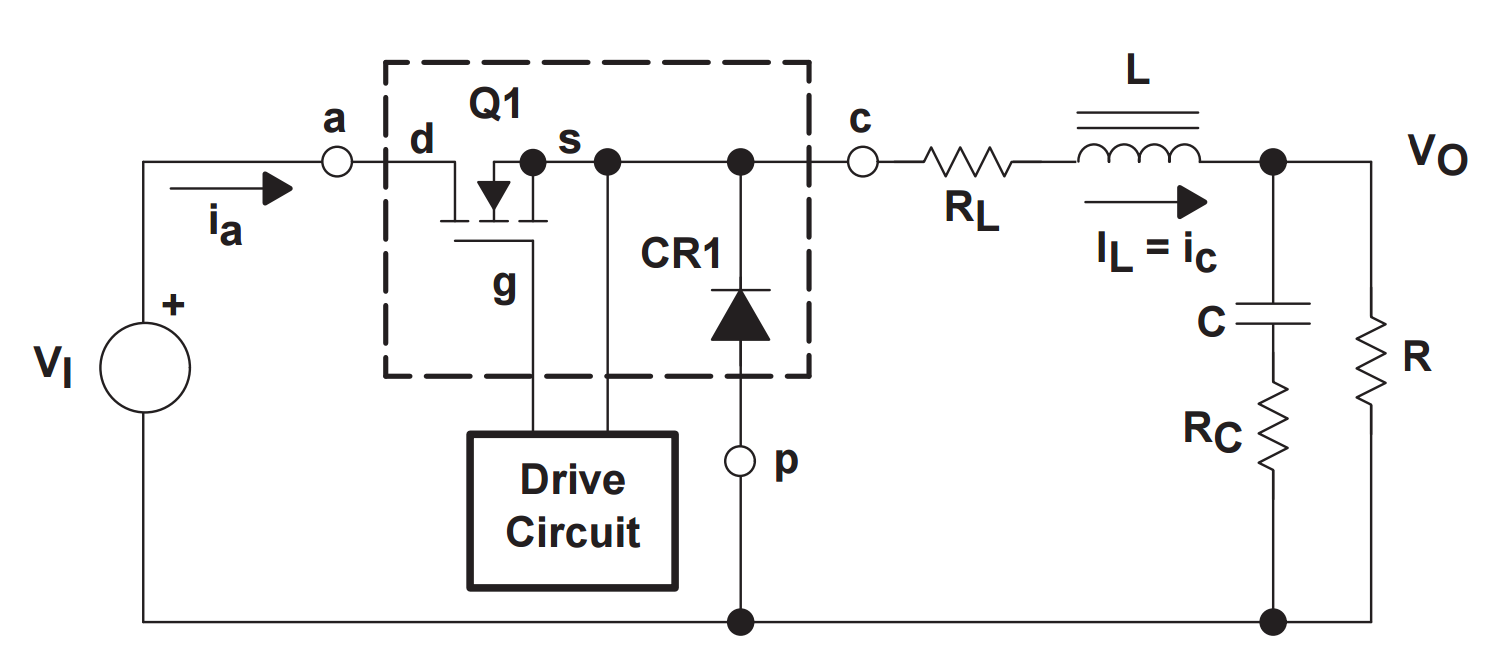
\includegraphics[width=\textwidth,height=\textheight,keepaspectratio]{buck_control_diagram}
		\caption{Diagrama de un convertidor tipo Buck}
		\label{buck:diagram}
	\end{figure}

	Podemos simplificar aún más el diagrama analizándolo en los dos estados del convertidor, cuando Q1 conduce y mientras no lo hace, los que llamaremos estados ON y OFF:
	
	\begin{figure}[H]
		\centering
		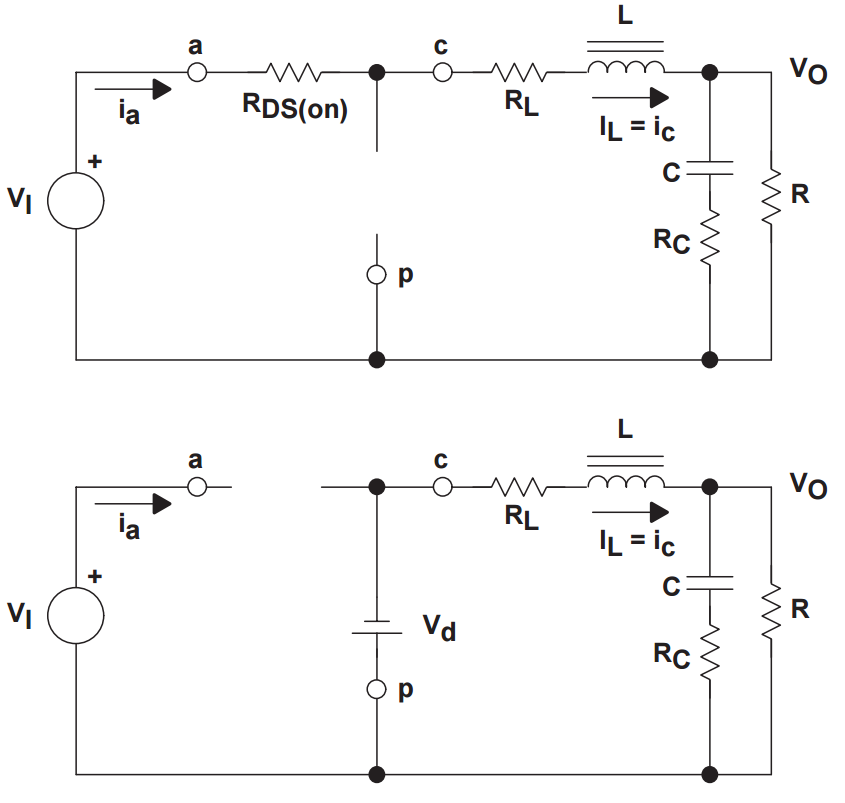
\includegraphics[width=\textwidth,height=\textheight,keepaspectratio]{buck_control_on_off}
		\caption{Estados ON y OFF del convertidor Buck}
	\end{figure}

\section{Circuito equivalente de conmutación promediado}

	Para comenzar a modelar el convertidor Buck primero debemos linealizar los componentes cuyo comportamiento no es lineal, es decir, aquellos que en este caso son elementos de conmutación como el MOSFET y el diodo aquí llamado CR1 para no confundirlo con el duty cycle que será representado con la letra D. Vamos a reemplazar entonces lo que se encuentra dentro del cuadro con lineas intermitentes en la figura \ref{buck:diagram}, que es el circuito de conmutación, por un sistema equivalente linealizado. Si observamos la siguiente figura mostrando las formas de onda de corriente y tensión del convertidor:
	
	\begin{figure}[H]
		\centering
		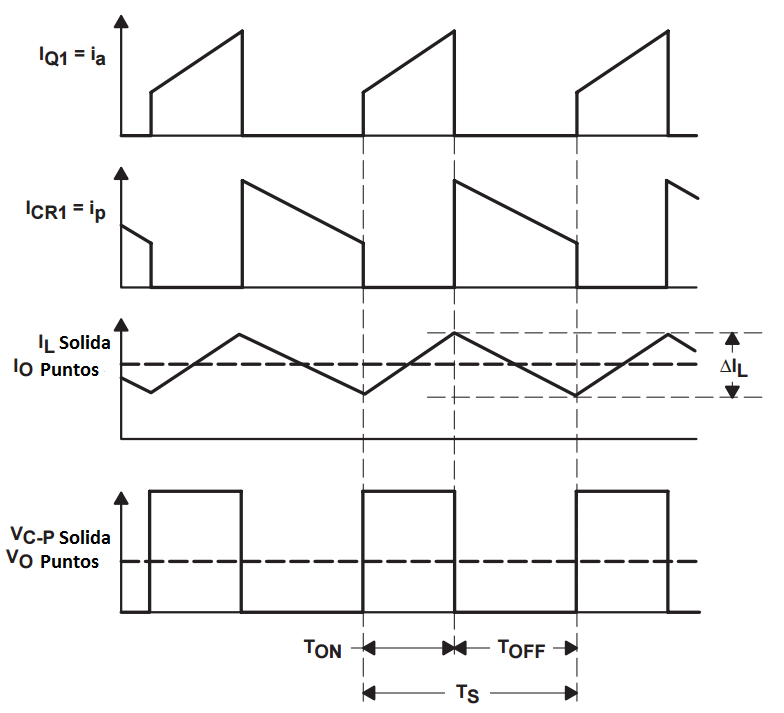
\includegraphics[width=\textwidth,height=\textheight,keepaspectratio]{buck_control_waveforms}
		\caption{Formas de onda del convertidor Buck}
	\end{figure}

	Podemos entonces formular las siguientes dos ecuaciones considerando que $d$ representa el duty cycle que varía entre 0 y 1:
	
	\begin{equation}
		i_{a(t)} = \left\{
		\begin{array}{ll}
			i_{c(t)} & durante \ d \cdot T_s \\
			0 & durante \ d' \cdot T_s
		\end{array}
		\right.
	\end{equation}
	
	\begin{equation}
		v_{cp(t)} = \left\{
		\begin{array}{ll}
			v_{ap(t)} & durante \ d \cdot T_s \\
			0 & durante \ d' \cdot T_s
		\end{array}
		\right.
	\end{equation}
	
	Donde $i_{a(t)}$ e $i_{c(t)}$ son las corrientes instantáneas durante un período $T_s$ y $v_{cp(t)}$ y $v_{ap(t)}$ son las tensiones instantáneas entre los puntos \textit{CP} y \textit{AP} respectivamente. Si tomamos entonces el promedio de cada una de estas ecuaciones podemos escribir que:
	
	\begin{equation}
		I_a = d \cdot I_c
		\label{equ:averaged_buck_current}
	\end{equation}
	
	\begin{equation}
		V_{cp} = d \cdot V_{ap}
		\label{equ:averaged_buck_voltage}
	\end{equation}
	
	Tomando como notación que las letras mayúsculas indican valores promedios o DC y las minúsculas aquellas que varían como el Duty Cycle $d$. Con estas expresiones podemos entonces reemplazar el bloque en línea de puntos que se mencionó antes de la siguiente forma:
	
	\begin{figure}[H]
		\centering
		\subfloat[Circuito original]{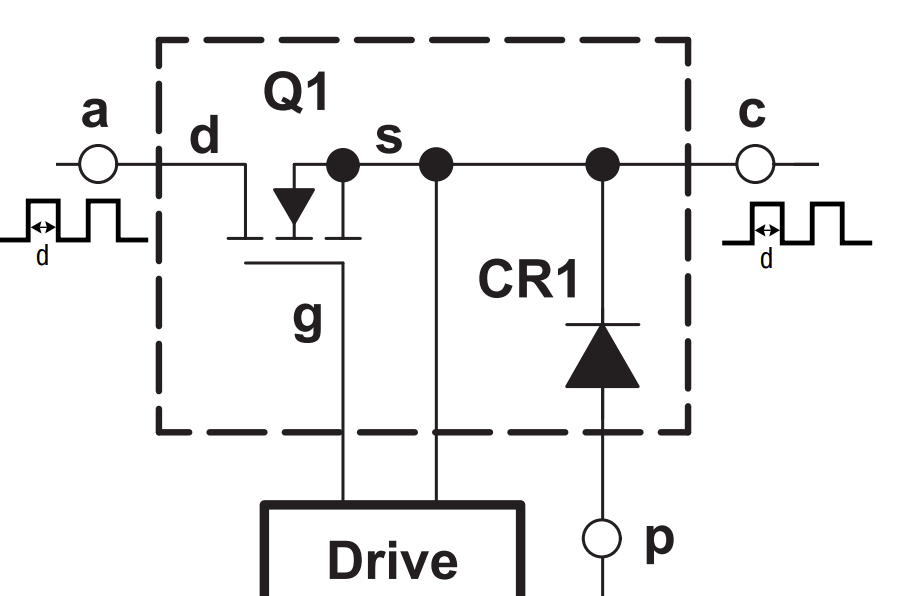
\includegraphics[width=0.47\textwidth]{buck_control_pwm_box}\label{fig:f1}}
		\hfill
		\subfloat[Circuito equivalente promedidado (no lineal)]{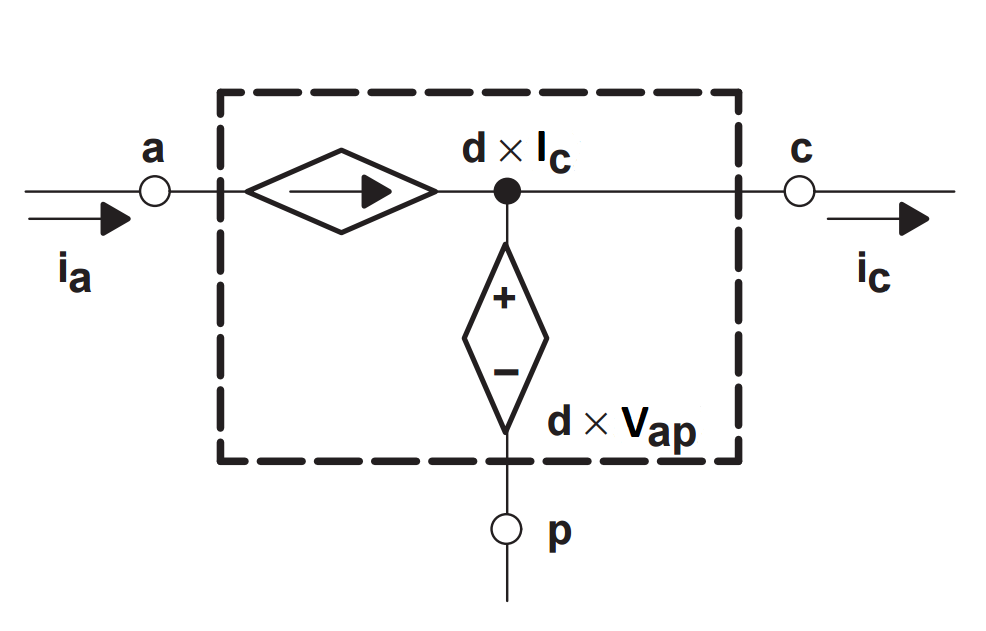
\includegraphics[width=0.47\textwidth]{buck_control_pwm_equivalent}\label{fig:f2}}
		\caption{Circuito equivalente promediado durante un período $T_s$}
	\end{figure}

	Donde se reemplaza el MOSFET y el diodo por una fuente de corriente y de tensión respectivamente. 
	
\section{Circuito equivalente de conmutación linealizado}

	El siguiente paso es realizar un proceso perturbación y linealización. La idea detrás del mismo es asumir un punto de operación e introducir pequeñas variaciones alrededor de ese punto para linealizar el sistema, es decir, decimos que el Duty se encuentra en un valor fijo D en estado estable y se le agrega al mismo una variación $\hat{d}(t)$, entonces:
	
	\begin{equation}
		d(t) = D + \hat{d}(t)
	\end{equation}
	
	Aplicamos así este proceso a las ecuaciones \ref{equ:averaged_buck_current} y \ref{equ:averaged_buck_voltage}:
	
	\begin{equation}
	\begin{aligned}
	I_a + \hat{i}_a(t) &= (D + \hat{d}(t)) \cdot (I_c + \hat{i}_c(t)) \\
		 &= D \cdot I_c + D \cdot \hat{i}_c(t) + \hat{d}(t) \cdot I_c + \hat{d}(t) \cdot \hat{i}_c(t) \\
	\end{aligned}
	\end{equation}
	
	\begin{equation}
	\begin{aligned}
	V_{cp} + \hat{v}_{cp}(t) &= (D + \hat{d}(t)) \cdot (V_{ap} + \hat{v}_{ap}(t)) \\
	&= D \cdot V_{ap} + D \cdot \hat{v}_{ap}(t) + \hat{d}(t) \cdot V_{ap} + \hat{d}(t) \cdot \hat{v}_{ap}(t) \\
	\end{aligned}
	\end{equation}
	
	Como las variaciones son pequeñas, el producto de dos variaciones pequeñas es aún más pequeño por lo que podemos eliminarlas:
	
	\begin{equation}
	\begin{aligned}
	I_a + \hat{i}_a(t) &= D \cdot I_c + D \cdot \hat{i}_c(t) + \hat{d}(t) \cdot I_c
	\end{aligned}
	\end{equation}
	
	\begin{equation}
	\begin{aligned}
	V_{cp} + \hat{v}_{cp}(t) &= D \cdot V_{ap} + D \cdot \hat{v}_{ap}(t) + \hat{d}(t) \cdot V_{ap}
	\end{aligned}
	\end{equation}
	
	Separamos entonces los términos constantes de los que presentan variación:
	
	\begin{enumerate}
		\item Términos constantes en el tiempo
			\subitem $I_a = D \cdot I_c$
			\subitem $V_{cp} = D \cdot V_{ap}$
		\item Términos variables en el tiempo
			\subitem $\hat{i}_a(t) = D \cdot \hat{i}_c(t) + \hat{d}(t) \cdot I_c$
			\subitem $\hat{v}_{cp}(t) = D \cdot \hat{v}_{ap}(t) + \hat{d}(t) \cdot V_{ap}$
	\end{enumerate}

	Si analizamos los términos constantes podemos realizar el siguiente circuito equivalente considerando un transformador ideal (independiente de la frecuencia) con una relación de transformación D:
	
	\begin{figure}[H]
		\centering
		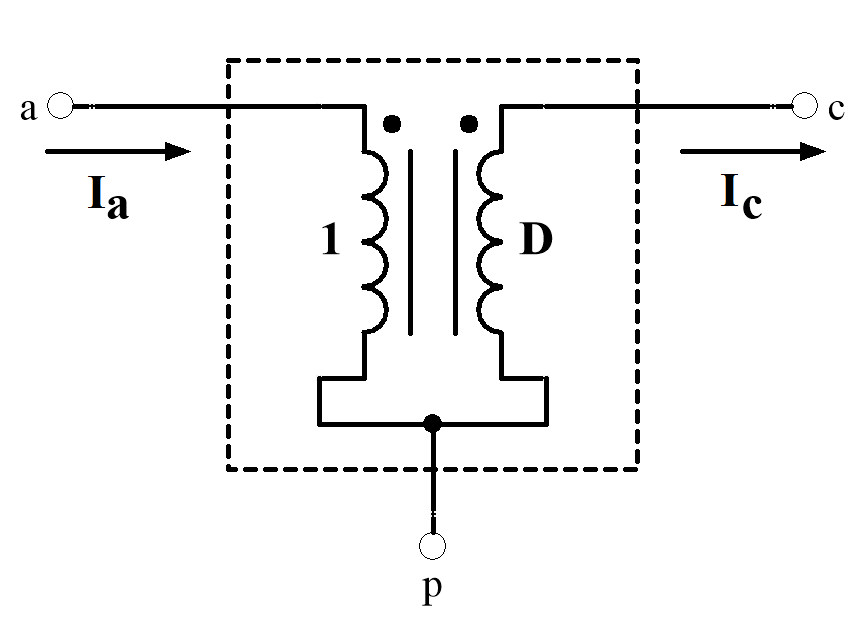
\includegraphics[width=0.5\textwidth,height=\textheight,keepaspectratio]{buck_control_dc_equivalent}
		\caption{Circuito equivalente en DC}
	\end{figure}

	Podemos ver que el circuito cumple con las dos ecuaciones constantes en el tiempo. Incorporamos ahora los términos variables y reflejando las fuentes al lado primario del transformador ideal tenemos:
	
	\begin{figure}[H]
		\centering
		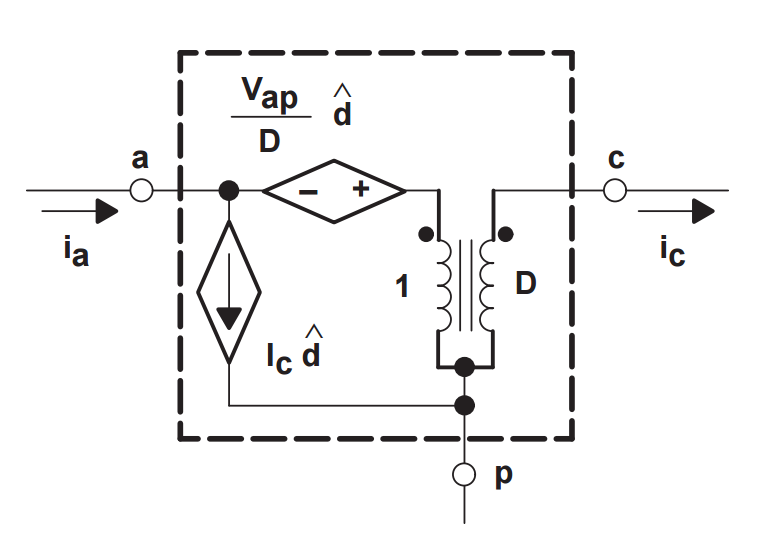
\includegraphics[width=0.9\textwidth,height=\textheight,keepaspectratio]{buck_control_dc_ac_equivalent}
		\caption{Circuito equivalente lineal y completo}
	\end{figure}

	De este modo el circuito cumple con las 4 ecuaciones y podemos finalmente reemplazar el bloque en el circuito de la figura \ref{buck:diagram} obteniendo un sistema lineal para el análisis:
	
	\begin{figure}[H]
		\centering
		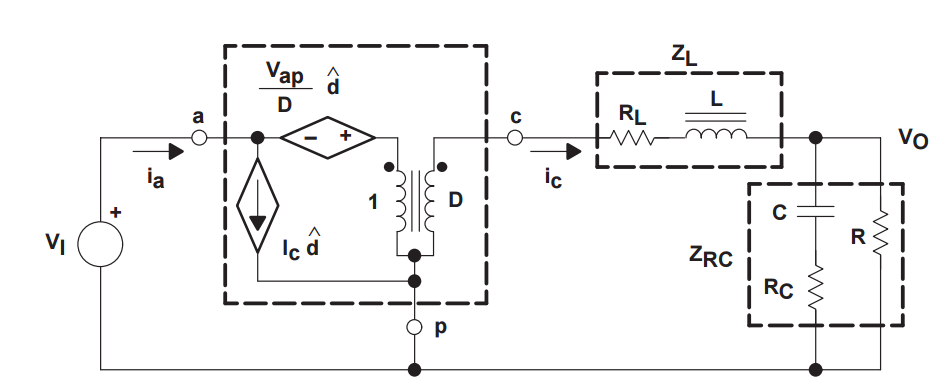
\includegraphics[width=0.9\textwidth,height=\textheight,keepaspectratio]{buck_control_full_equivalent}
		\caption{Convertidor buck linealizado}
	\end{figure}

\section{Determinación de la función de transferencia $H(S)$}

	Entonces para determinar ahora la función de transferencia del sistema cuya relación será $H_{(s)} = v_{o}(s)/\hat{d}(s)$, hacemos primero el análisis en DC para determinar el punto de operación D haciendo $\hat{d}(t) = 0$ y viendo de este modo que $V_{ap} = V_I$. 
	
	Luego hacemos $V_I = 0$ para tener únicamente la componente AC de la función de transferencia y escribimos la ecuación de malla del primario:
	
	\begin{equation}
	\begin{aligned}
	-\dfrac{V_{ap}}{D} \cdot \hat{d}(t) + \dfrac{\hat{v}_{cp}(t)}{D} = 0 \ \therefore \ \hat{v}_{cp}(t) = V_{ap} \cdot \hat{d}(t) \ \therefore \ \Aboxed{\hat{v}_{cp}(t) = V_I \cdot \hat{d}(t)}
	\end{aligned}
	\end{equation}
	
	O de otra forma:
	
	\begin{equation}
	\dfrac{\hat{v}_{cp}(s)}{\hat{d}(s)} = V_I
	\end{equation}
	
	Y sabiendo que la función de transferencia entre la tensión de salida y $v_{cp}$ es (tratándolo como un divisor de tensión de impedancias):
	
	\begin{equation}
	\dfrac{\hat{v_o}(s)}{\hat{v}_{cp}(s)} = \dfrac{Z_{RC}(s)}{Z_{RC}(s) + Z_L(s)}
	\end{equation}
	
	En donde $Z_L(t)$ es:
	
	\begin{equation}
	\begin{aligned}
	Z_L(t) = R_L + j\omega \cdot L \ \therefore \ \Aboxed{Z_L(s) = R_L + s \cdot L}
	\end{aligned}
	\end{equation}
	
	Y donde $Z_{RC}$ es:
	
	\begin{equation}
	\begin{aligned}
	Z_{RC} 	&= \left(\dfrac{1}{j \omega C} + R_C \right) \parallel R \\ \\
			&= \dfrac{\left(\dfrac{1}{j \omega C} + R_C \right) \cdot R}{\dfrac{1}{j \omega C} + R_C + R} \\ \\
			&= \dfrac{\dfrac{R}{sC} + R_C \cdot R}{\dfrac{1}{sC} + R_C + R} \\ \\
			&= \dfrac{ \dfrac{R + s \cdot C \cdot R_C \cdot R}{\cancel{s \cdot C}} }{ \dfrac{1 + s \cdot C \cdot R_C + s \cdot C \cdot R}{\cancel{s \cdot C}} } \\ \\
			&= \dfrac{R + s \cdot C \cdot R_C \cdot R}{1 + s \cdot C \cdot R_C + s \cdot C \cdot R} = \Aboxed{\dfrac{R \cdot (1 + s \cdot C \cdot R_C)}{1 + s \cdot C \cdot (R_C + R)}}
	\end{aligned}
	\end{equation}
	
	Por lo tanto:
	
	\begin{align*}
	\dfrac{\hat{v_o}(s)}{\hat{v}_{cp}(s)} &= \dfrac{\dfrac{R \cdot (1 + s \cdot C \cdot R_C)}{1 + s \cdot C \cdot (R_C + R)}}{ \dfrac{R \cdot (1 + s \cdot C \cdot R_C)}{1 + s \cdot C \cdot (R_C + R)} + R_L + s \cdot L } \\
	&= \dfrac{\dfrac{A}{B}}{\dfrac{A}{B} + R_L + s \cdot L} \\
	&= \dfrac{\dfrac{A}{\cancel{B}}}{\dfrac{A + R_L \cdot B + s \cdot L \cdot B}{\cancel{B}}} \\
	&= \dfrac{A}{A + R_L \cdot B + s \cdot L \cdot \underbrace{(1 + s \cdot F \cdot (R_C + R))}_\text{B}} \tag{\stepcounter{equation}\theequation} \\
	&= \dfrac{A}{A + R_L \cdot B + s \cdot L + s^2 \cdot L \cdot C \cdot (R + R_C)} \\ \\
	&= \dfrac{R + s \cdot R \cdot R_C \cdot C}{\displaystyle{(R + s \cdot R \cdot R_C \cdot C) + (R_L + R_L \cdot s \cdot C \cdot (R + R_C)) + \atop \hfill s \cdot L + s^2 \cdot L \cdot C \cdot (R + R_C)}} \\ \\
	&= \Aboxed{\dfrac{R + s \cdot R \cdot R_C \cdot C}{s^2 \cdot [L \cdot C \cdot (R + R_C)] + s \cdot [R \cdot R_C \cdot C + R_L \cdot C \cdot (R + R_C) + L] + (R + R_L)}}
	\end{align*}
	
	Finalmente podemos reemplazar y escribir la función de transferencia $\hat{v_o}(s)/\hat{d}(s)$:
	
	\begin{equation}
	\begin{aligned}
	&H(S) = \dfrac{\hat{v_o}(s)}{\hat{d}(s)} = \dfrac{\hat{v}_{cp}(s)}{\hat{d}(s)} \cdot \dfrac{\hat{v_o}(s)}{\hat{v}_{cp}(s)} \\	
	&=\Aboxed{V_I \cdot \dfrac{R + s \cdot R \cdot R_C \cdot C}{s^2 \cdot [L \cdot C \cdot (R + R_C)] + s \cdot [R \cdot R_C \cdot C + R_L \cdot C \cdot (R + R_C) + L] + (R + R_L)}}
	\end{aligned}
	\end{equation}
	
\section{Cálculo de los parámetros PID en MATLAB\textregistered}

	\lstset{language=Matlab,%
		%basicstyle=\color{red},
		backgroundcolor = \color{codebg},
		inputencoding=utf8/latin1,
		breaklines=true,%
		morekeywords={matlab2tikz},
		keywordstyle=\color{blue},%
		morekeywords=[2]{1}, keywordstyle=[2]{\color{black}},
		identifierstyle=\color{black},%
		stringstyle=\color{mylilas},
		commentstyle=\color{mygreen},%
		showstringspaces=false,%without this there will be a symbol in the places where there is a space
		numbers=left,%
		numberstyle={\color{black}},% size of the numbers
		numbersep=9pt, % this defines how far the numbers are from the text
		emph=[1]{for,end,break},emphstyle=[1]\color{red}, %some words to emphasise
		%emph=[2]{word1,word2}, emphstyle=[2]{style},    
	}

	Insertamos ahora nuestra función de transferencia $H(s)$ en MATLAB\textregistered utilizando el siguiente programa: 

	\begin{minipage}{\textwidth}
		\lstinputlisting{../Matlab/PID.m}
	\end{minipage}
	
	Usamos entonces la herramienta \textit{PID Tuner} de MATLAB\textregistered, seleccionamos un control del tipo PID y ajustamos los controles \textit{Tiempo de respuesta} y \textit{Respuesta a transitorios} hasta obtener una curva que nos convenza, en nuestro caso se priorizó la eliminación de sobre-elongaciones antes que el tiempo de establecimiento del sistema como se muestra en la figura \ref{buck:settling_time}
	
	\begin{sidewaysfigure}
		\centering
		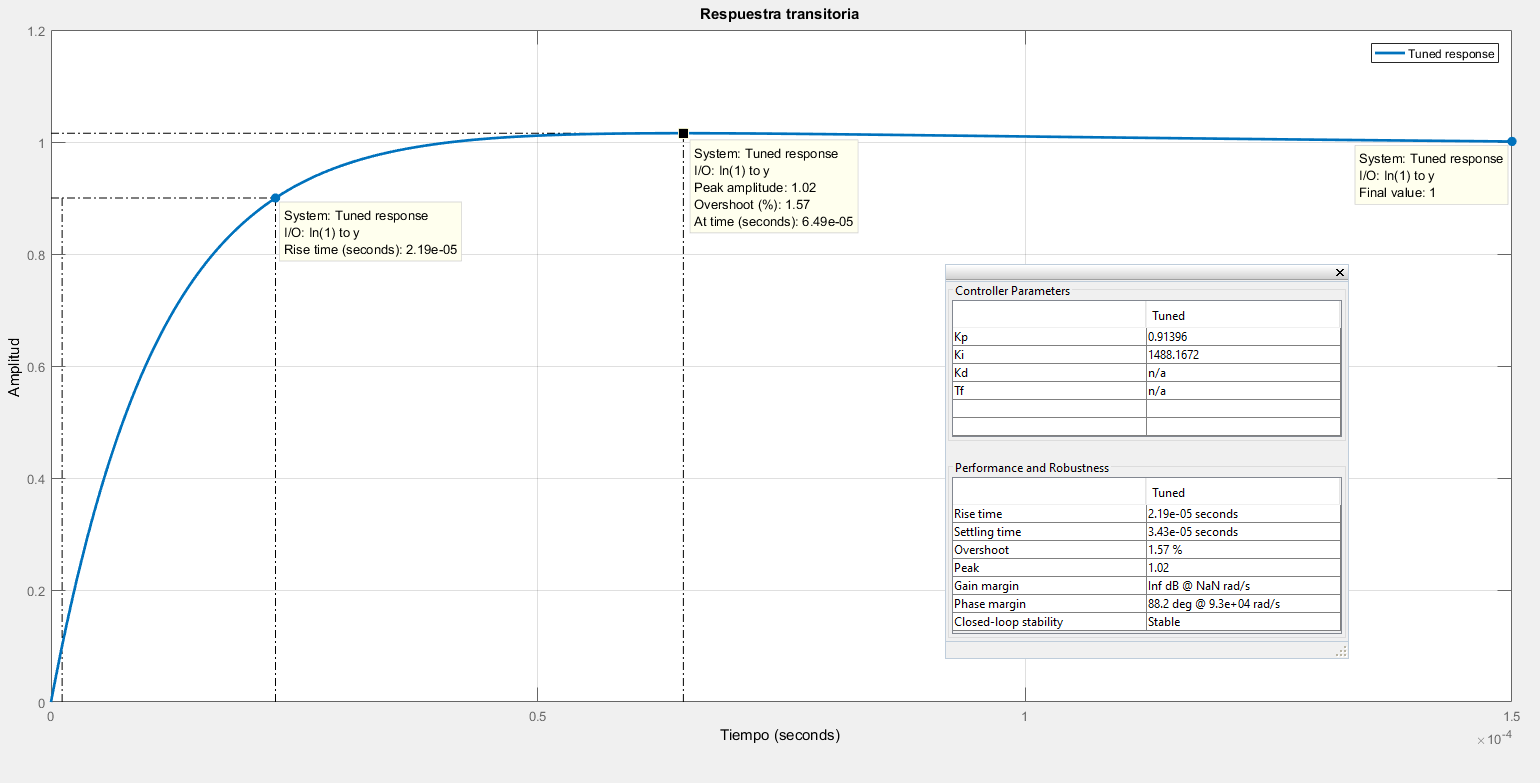
\includegraphics[width=\textwidth,height=\textheight,keepaspectratio]{buck_step_response} 
		\caption{Respuesta transitoria de lazo cerrado}
		\label{buck:settling_time}
	\end{sidewaysfigure}

	\newpage
	Ya habiendo entonces obtenido los valores de Kp, Ki y Kd podemos obtener las distintas repuestas de nuestro sistema tanto en el plano continuo como en el discreto.

	\subsection{Análisis en el plano continuo s}
	
	El siguiente programa de MATLAB\textregistered \ fue usado para los análisis de respuesta transitoria, estado estable, Bode, Nyquist y diagrama de polos y ceros teniendo ya los valores de Kp, Ki y Kd. Este programa utiliza además la función de la planta $G(s)$ del programa anterior:
	
	\lstinputlisting{../Matlab/Plots_continuo.m}
	
	\subsubsection{Respuesta transitoria}
	
	En la figura \ref{buck:settling_time} se observa la respuesta al escalón unitario del sistema de lazo cerrado. Podemos ver que el tiempo de crecimiento es de $192 \mu s$ y el tiempo de establecimiento de $330 \mu s$ sin sobre-elongación de ningún tipo. 
	
	El margen de fase es de 90 grados lo que significa que podemos introducir un defasaje de hasta dicho ángulo en el lazo de control sin perder la estabilidad del sistema.
	
	\subsubsection{Estado Estacionario}
	
	En la figura \ref{buck:steady_state} podemos observar que no tenemos error de estado estable, es decir, el controlador alcanza el setpoint y no presenta ningún comportamiento oscilatorio.
	
	\subsubsection{Respuesta en frecuencia}

	En la figura \ref{buck:bode} se puede apreciar como el ancho de banda de nuestro sistema se encuentra alrededor de los 194 KHz donde tenemos una caída de -3dB, esta frecuencia se encuentra dentro del rango de nuestra frecuencia de conmutación por lo que es importante considerar un buen filtrado de cualquier ruido de conmutación que pueda perturbar al lazo de realimentación ya que el sistema sería capaz de responder a los mismos.
	
	El margen de fase es de -180 grados lo que indica que podemos agregar hasta 180 de fase a nuestro sistema sin volverlo inestable. Respecto al margen de ganancia, el mismo es infinito lo que significa que en teoría podríamos agregar tanta ganancia como quisiéramos sin volver inestable al sistema.
	
	\subsubsection{Diagrama de polos y ceros}

	En la figura \ref{buck:polos_ceros} se presenta el diagrama de polos y ceros. Debido a que las distancias entre los distintos polos y ceros son variadas y no están concentrados en un punto resulta quizás más útil observar el resultado proveniente de la función \textit{pzmap()} de MATLAB\textregistered donde muestra los valores numéricos de los distintos polos y ceros:
	
	\begin{itemize}
		\item Polos:
			\subitem \num{-1.2079e6}
			\subitem \num{-2120}
			\subitem \num{-546}
		\item Ceros:
			\subitem \num{-2120}
			\subitem \num{-546}
	\end{itemize}
	
	Podemos ver que tanto los polos como ceros se encuentran en el eje real y del lado negativo por lo que el sistema es estable y dado a que se encuentran distribuidos a lo largo del eje el sistema es sobre-amortiguado.
	
	%\subsubsection{Diagrama de Nyquist}
	%Figura \ref{buck:nyquist} % TODO: Hacer analisis de Nyquist

	\begin{sidewaysfigure}
		\centering
		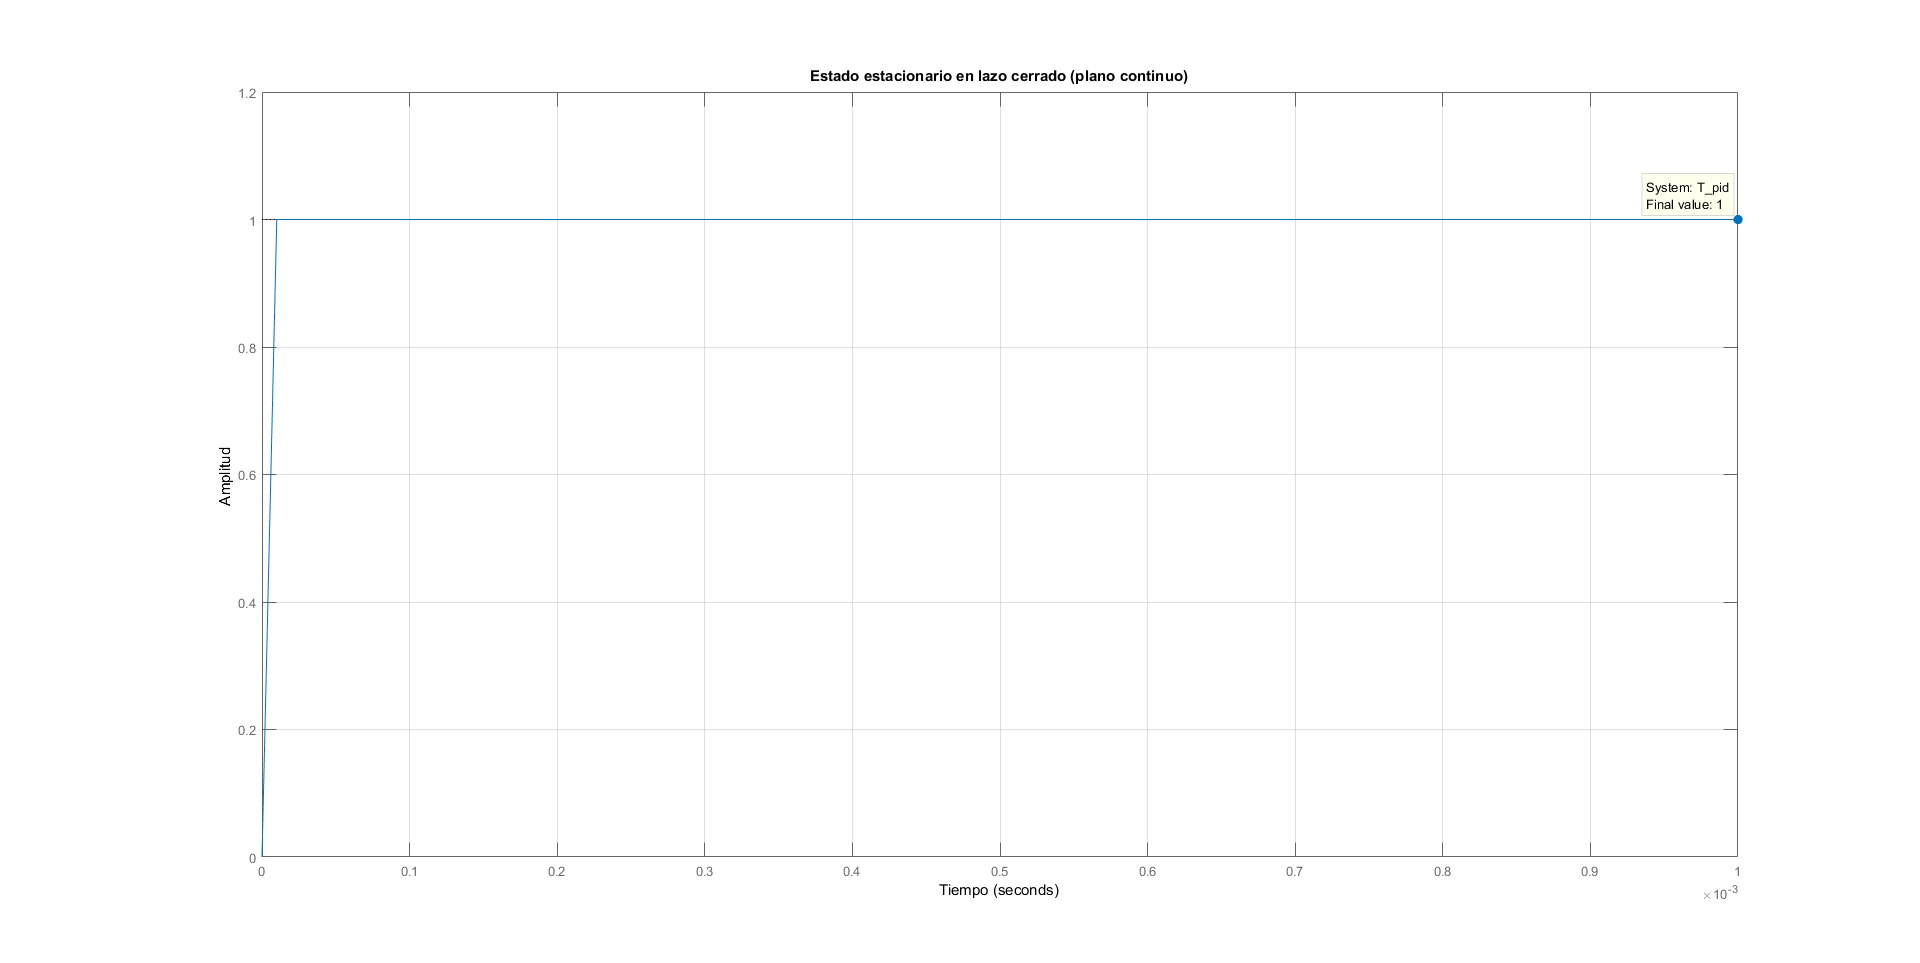
\includegraphics[width=\textwidth,height=\textheight,keepaspectratio]{buck_steady_state} 
		\caption{Estado estacionario}
		\label{buck:steady_state}
	\end{sidewaysfigure}
	
	\begin{sidewaysfigure}
		\centering
		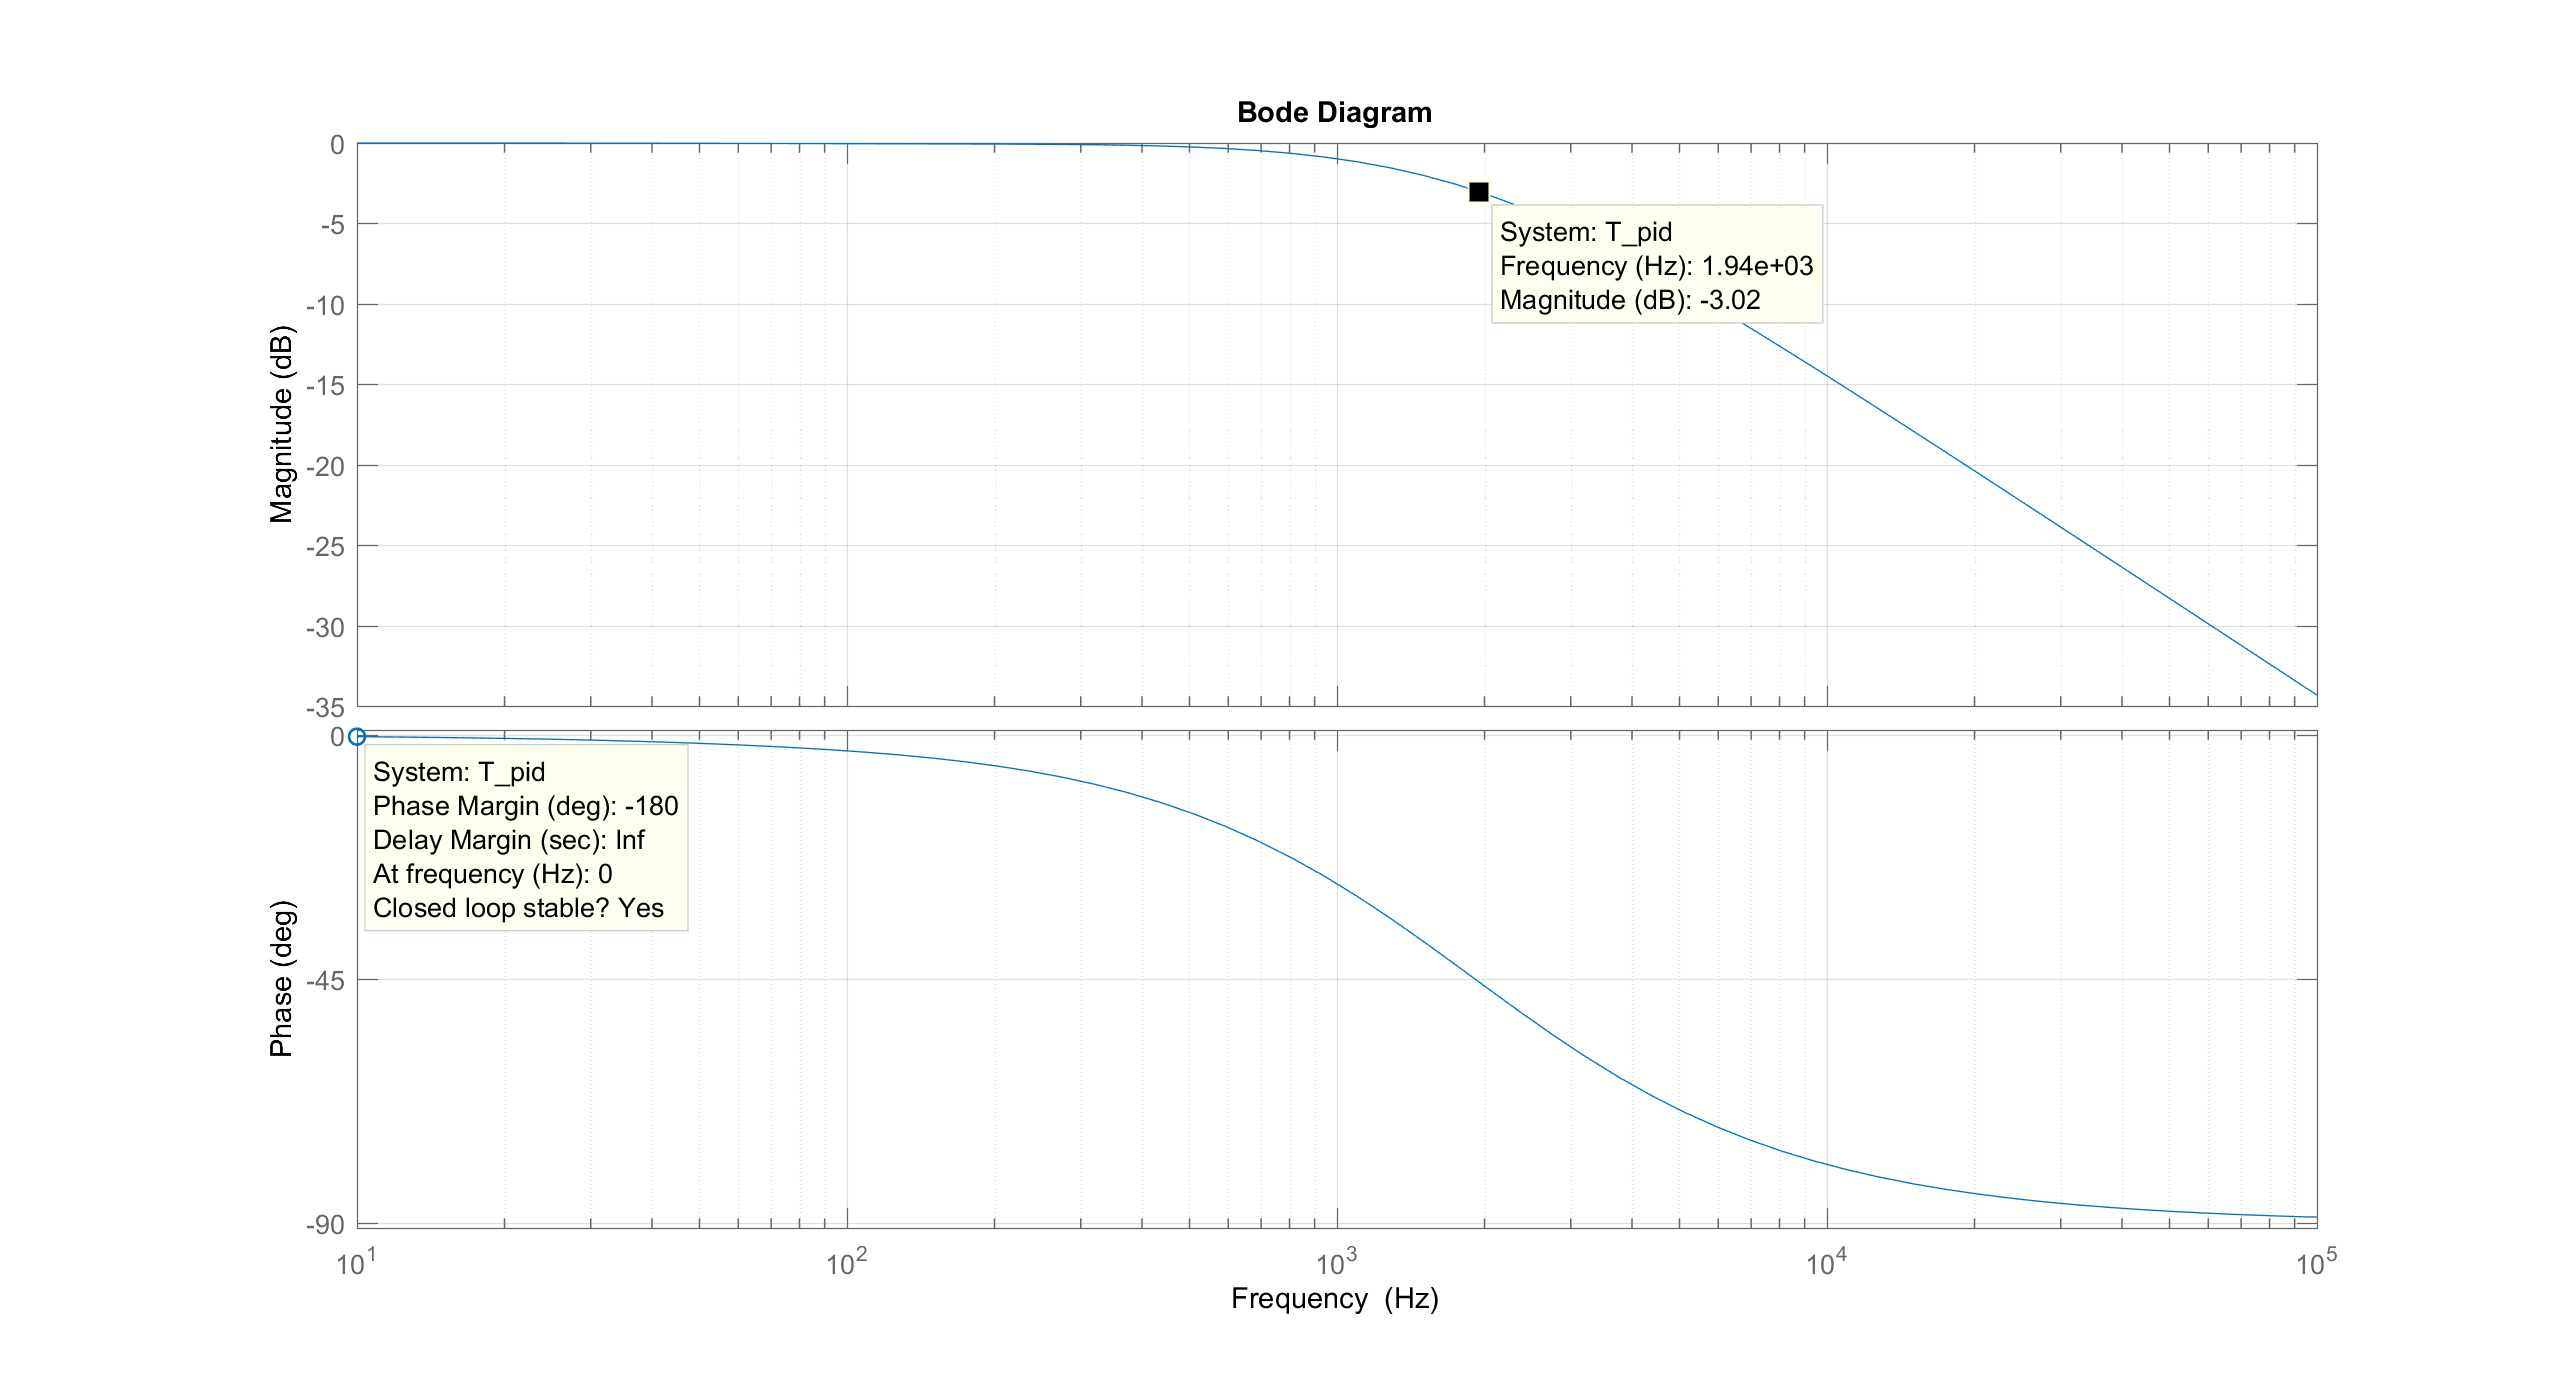
\includegraphics[width=\textwidth,height=\textheight,keepaspectratio]{buck_bode} 
		\caption{Respuesta en frecuencia - Diagrama de Bode}
		\label{buck:bode}
	\end{sidewaysfigure}
	
	\begin{sidewaysfigure}
		\centering
		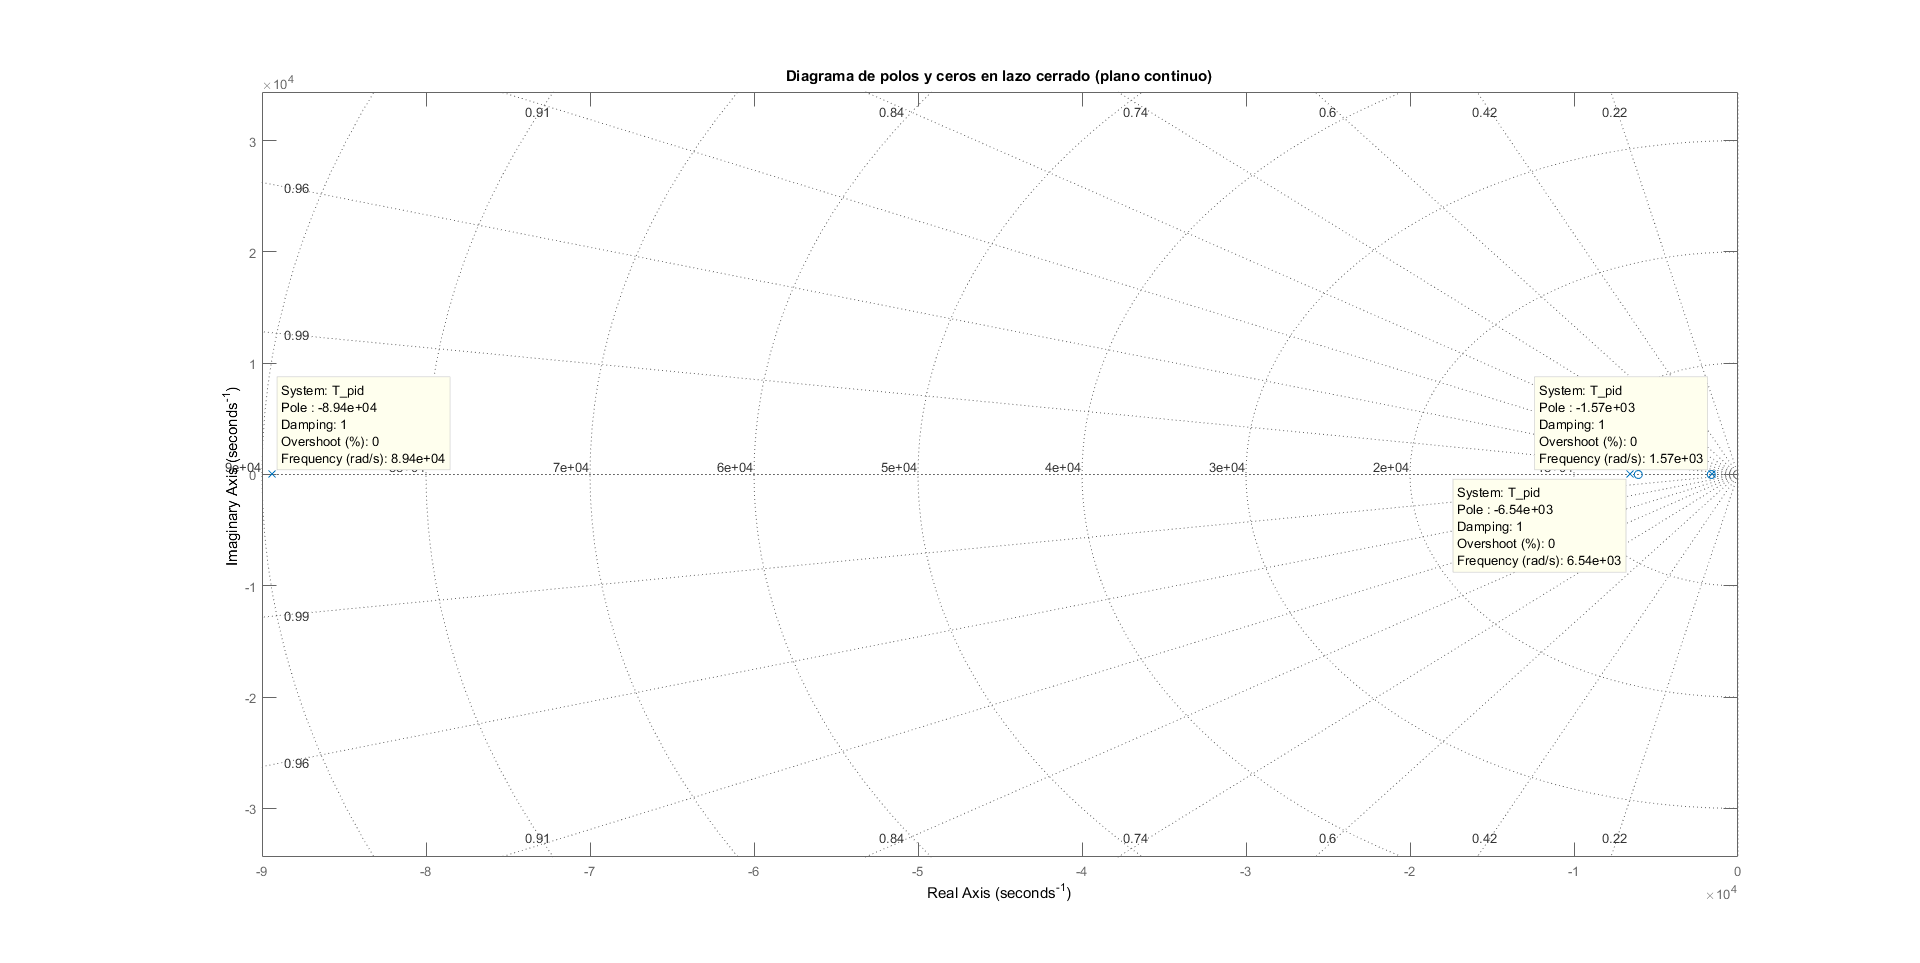
\includegraphics[width=\textwidth,height=\textheight,keepaspectratio]{buck_polos_ceros} 
		\caption{Diagrama de polos y ceros}
		\label{buck:polos_ceros}
	\end{sidewaysfigure}

	\begin{sidewaysfigure}
		\centering
		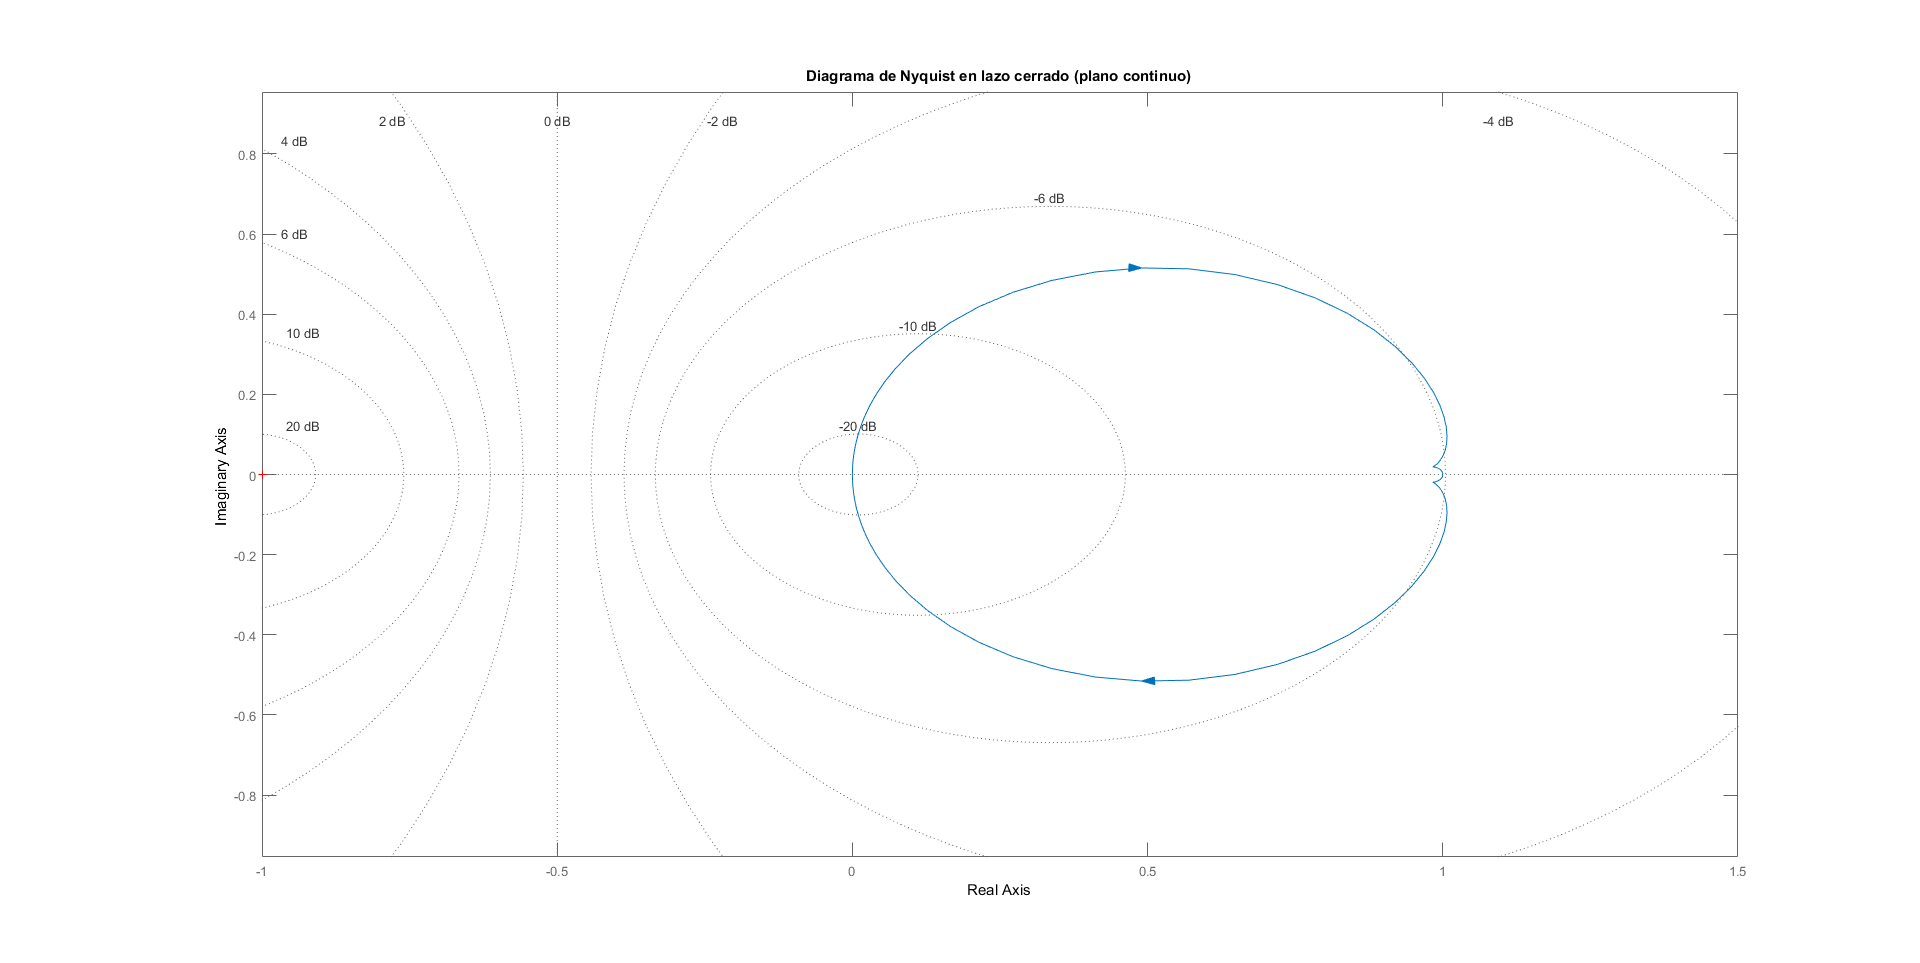
\includegraphics[width=\textwidth,height=\textheight,keepaspectratio]{buck_nyquist} 
		\caption{Diagrama de Nyquist}
		\label{buck:nyquist}
	\end{sidewaysfigure}

	\newpage
	\subsection{Análisis en el plano discreto z}

	Para el análisis en el plano discreto se discretizó el sistema con la frecuencia de muestreo del ADC del DSP que es de 2 MSPS. El siguiente programa de MATLAB\textregistered \ fue el utilizado para el análisis:
	
	\lstinputlisting{../Matlab/Plots_discreto.m}
	
	En nuestro caso las observaciones del sistema tienen más sentido sobre el plano z ya que nuestro sistema es discreto y no continuo, debido a que se muestrea la señal de realimentación. 
	
	\subsubsection{Respuesta transitoria}
	
	En la figura \ref{buck:step_discrete} se observa la respuesta al escalón unitario del sistema de lazo cerrado. Podemos ver que la respuesta es muy similar o idéntica a la obtenida en el plano continuo. Esto es un buen indicador ya que significa que la frecuencia de muestreo es lo suficientemente alta como para controlar el sistema de manera adecuada. Por ejemplo, si utilizamos una frecuencia baja como 2 kHz la respuesta que tenemos es la siguiente:
	
	\begin{figure}[H]
		\centering
		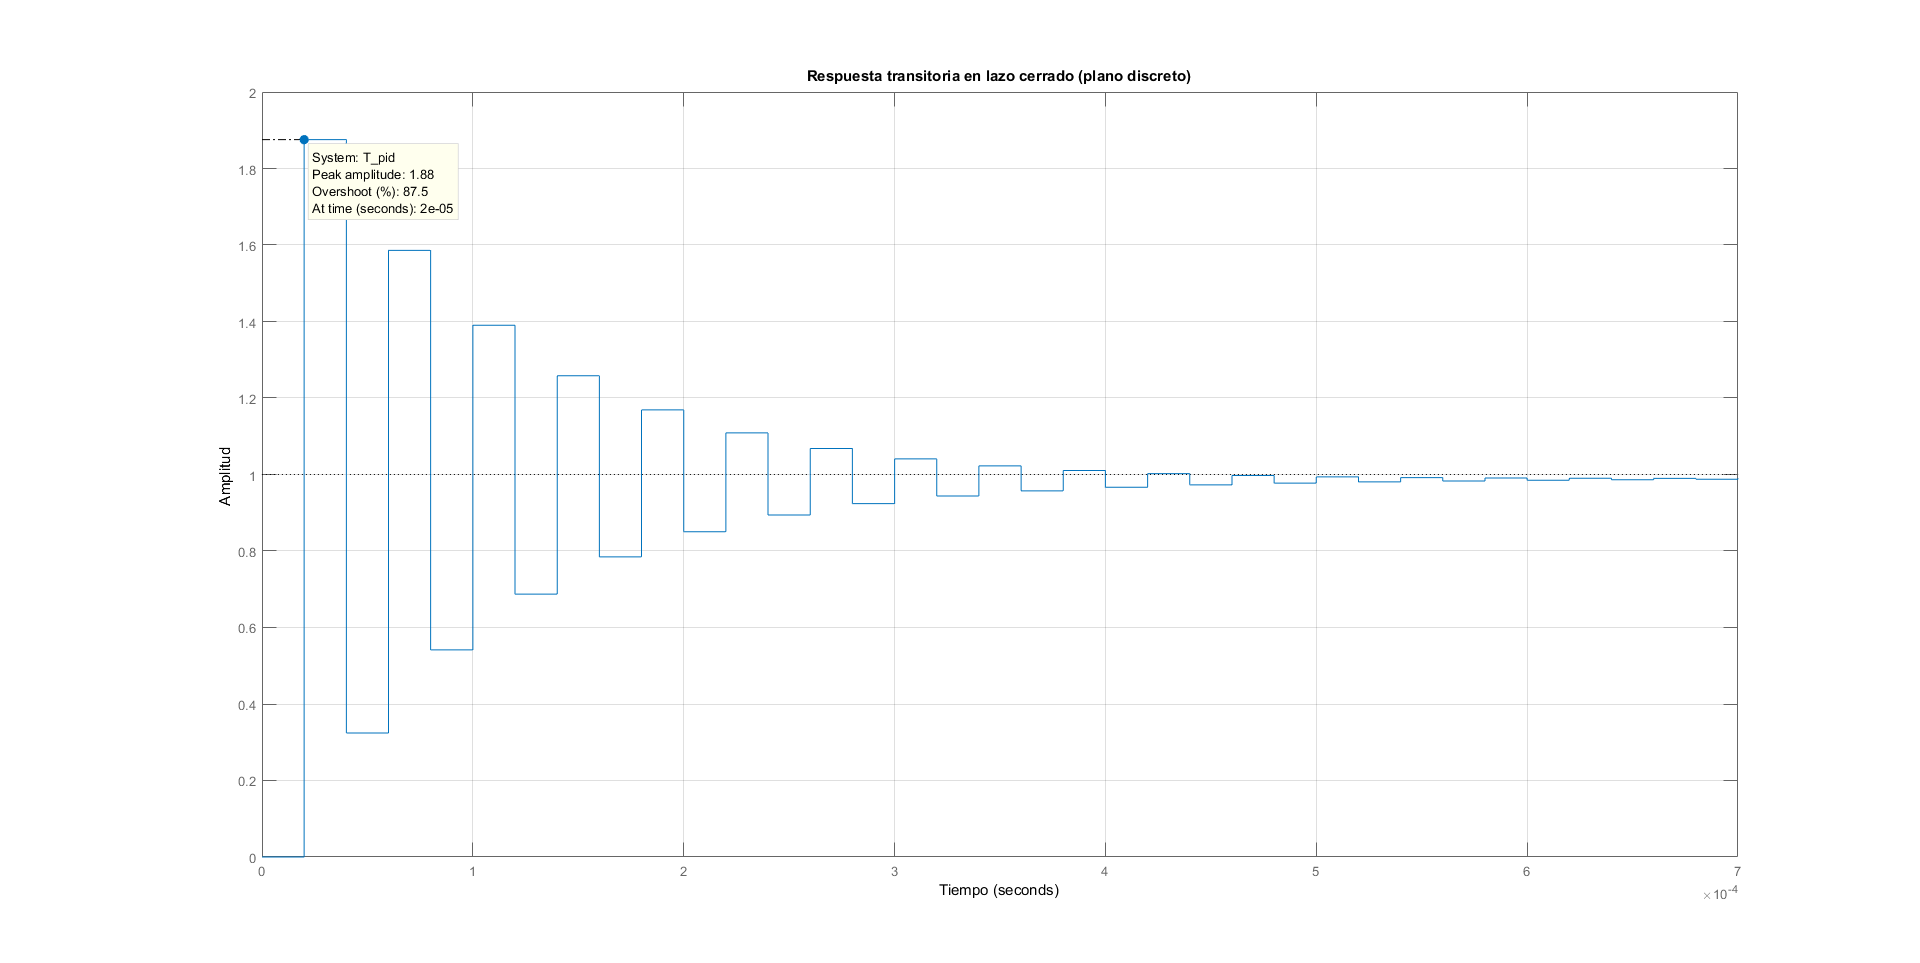
\includegraphics[width=0.9\textwidth,height=\textheight,keepaspectratio]{buck_step_low_freq}
		\caption{Respuesta transitoria con baja frecuencia de muestreo}
	\end{figure}
	
	\subsubsection{Estado Estacionario}
	
	En las figura \ref{buck:steady_state_discrete} vemos que el sistema se comporta de la misma manera que lo hacía en el plano continuo s.
	
	\subsubsection{Respuesta en frecuencia}
	
	Observando la figura \ref{buck:bode_discrete} vemos como el ancho de banda del sistema se redujo drásticamente a 2 kHz con respecto a los casi 200 kHz obtenidos en el plano continuo. El margen de fase se mantuvo en -180 grados y el de ganancia ya no es infinito sino que pasa a ser de 27.6dB lo que nos indica que ésta es la ganancia máxima que podemos agregar al sistema sin volverlo inestable.
	
	\subsubsection{Diagrama de polos y ceros}
	
	En la figura \ref{buck:polos_ceros_discrete} vemos los polos y ceros no se encuentran en los mismos lugares pero todos son reales y negativos por lo que el sistema sigue siendo estable y sobre-amortiguado.
	
	\begin{sidewaysfigure}
		\centering
		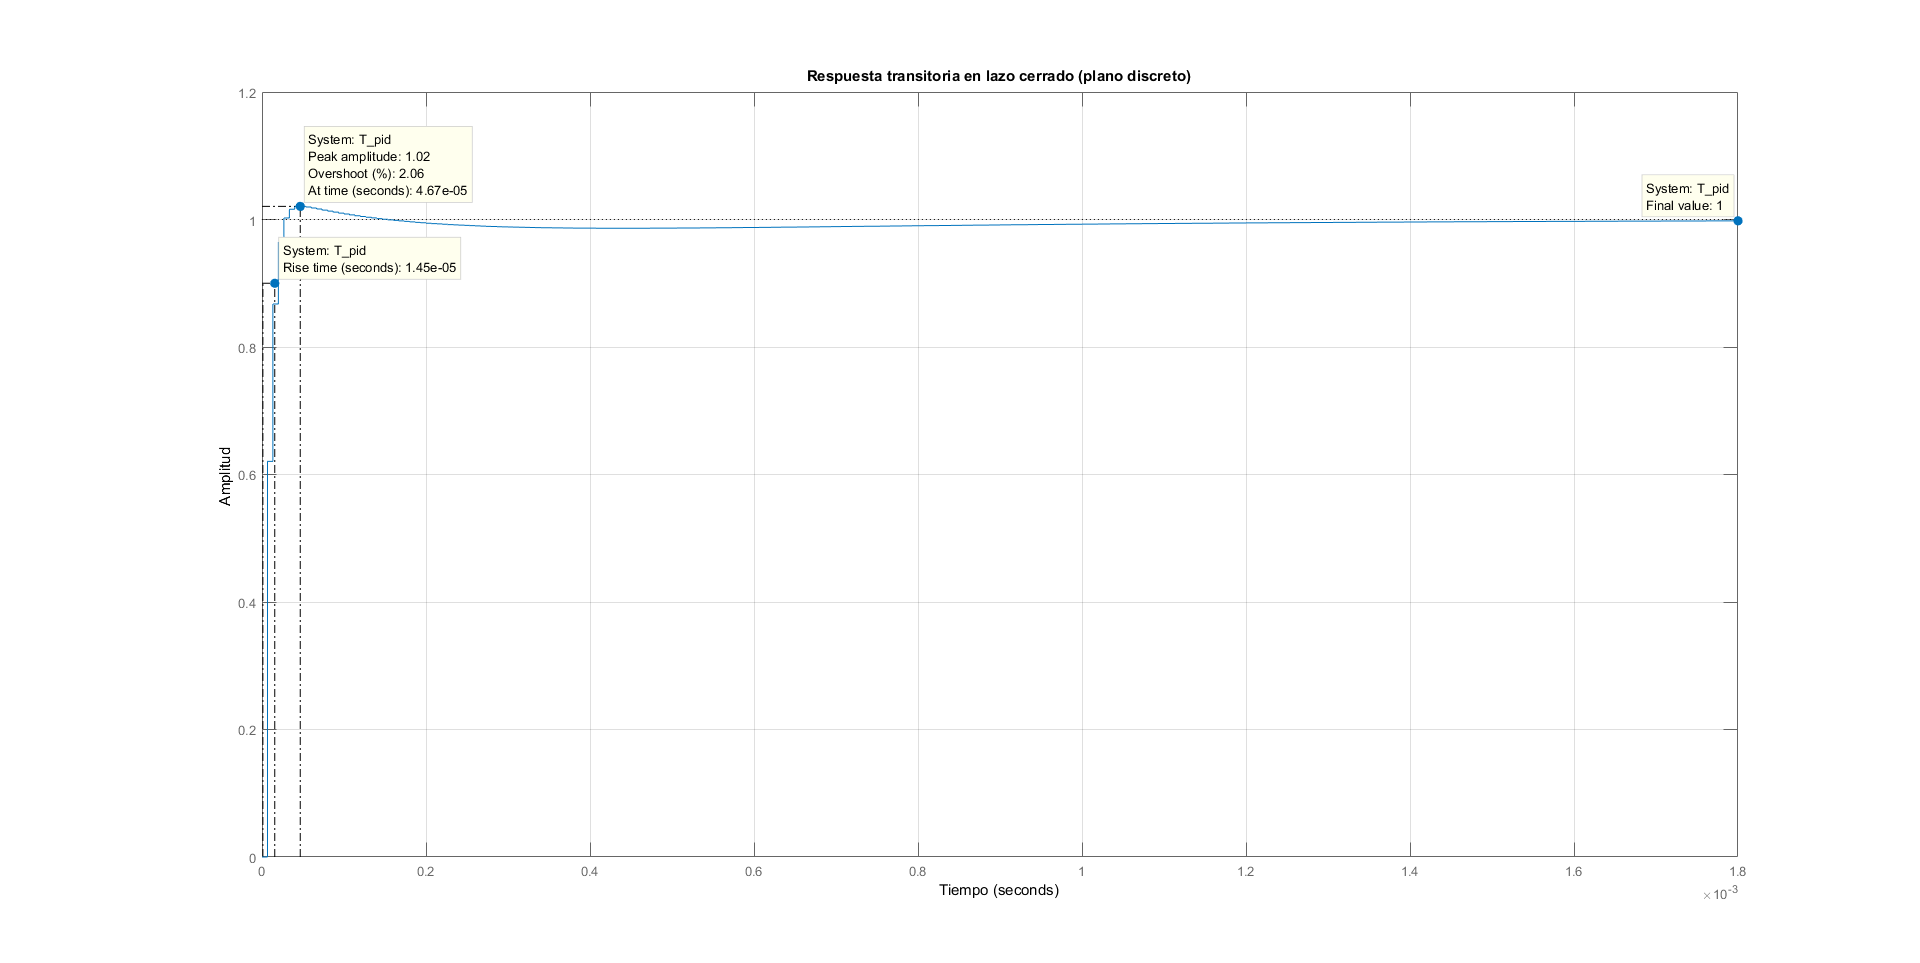
\includegraphics[width=\textwidth,height=\textheight,keepaspectratio]{buck_step_response_discrete} 
		\caption{Respuesta transitoria - Sistema Discreto}
		\label{buck:step_discrete}
	\end{sidewaysfigure}
	
	\begin{sidewaysfigure}
		\centering
		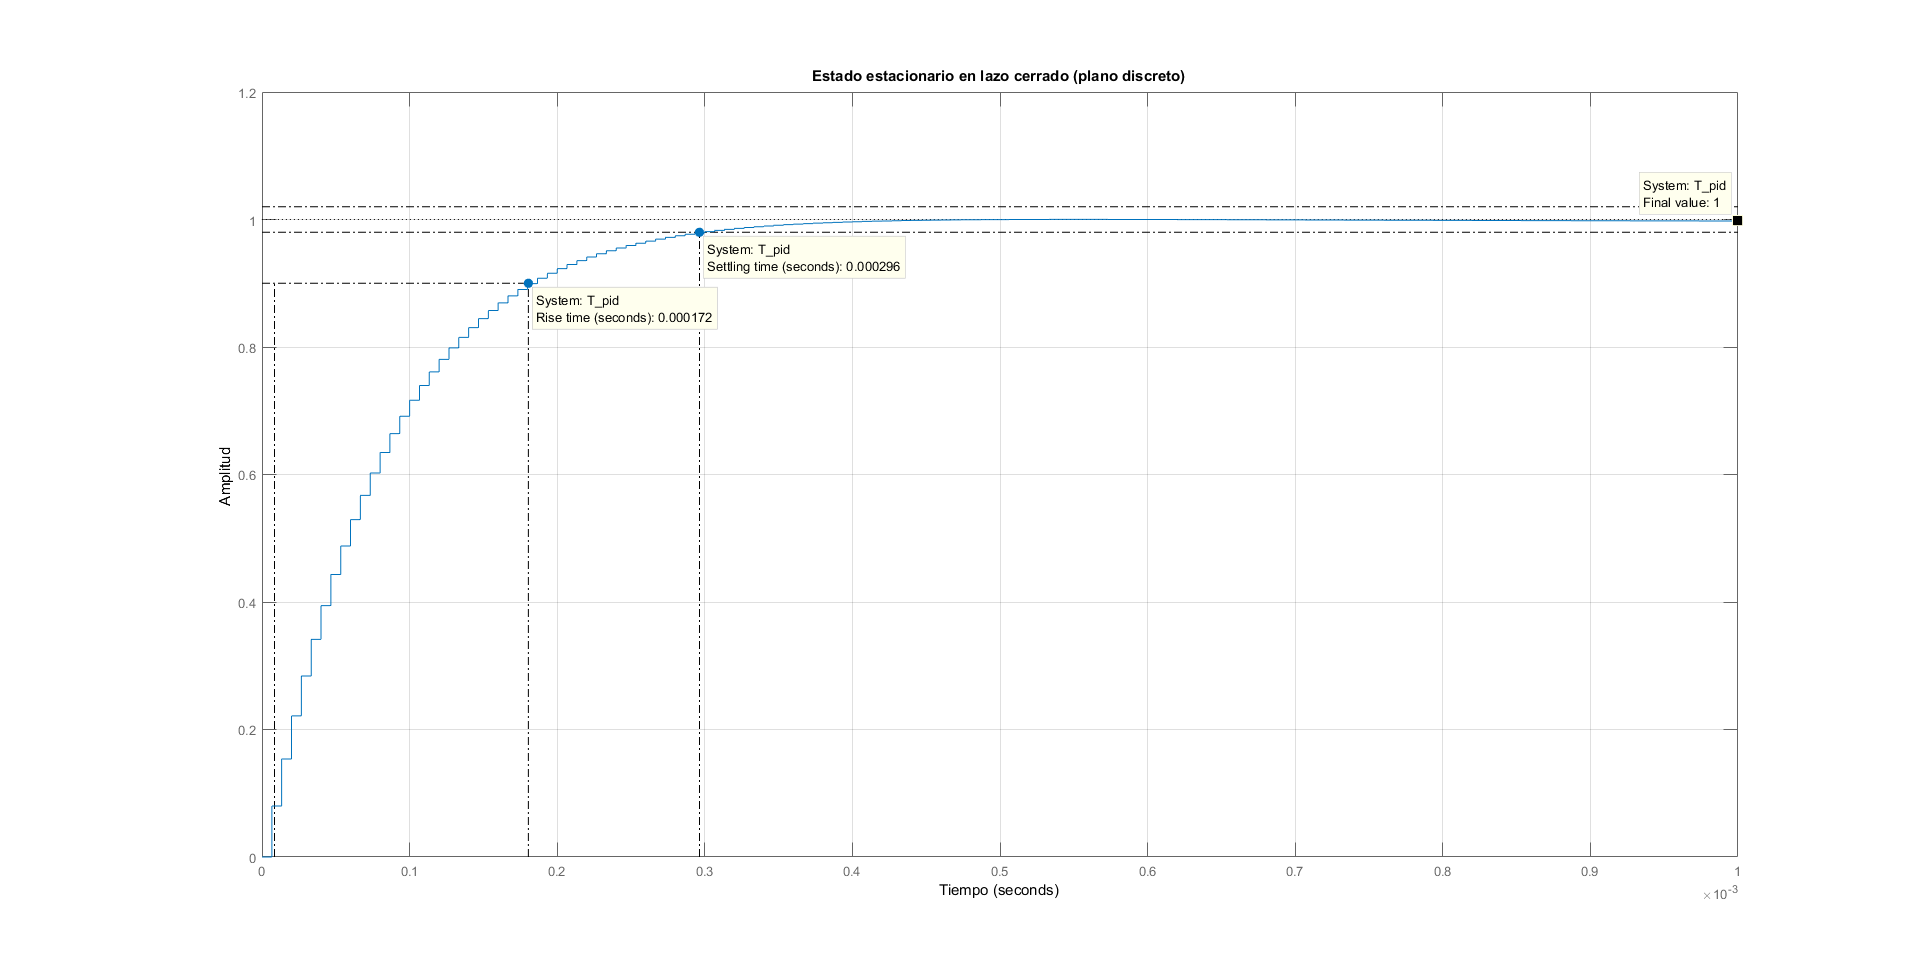
\includegraphics[width=\textwidth,height=\textheight,keepaspectratio]{buck_steady_state_discrete} 
		\caption{Estado estacionario - Sistema Discreto}
		\label{buck:steady_state_discrete}
	\end{sidewaysfigure}
	
	\begin{sidewaysfigure}
		\centering
		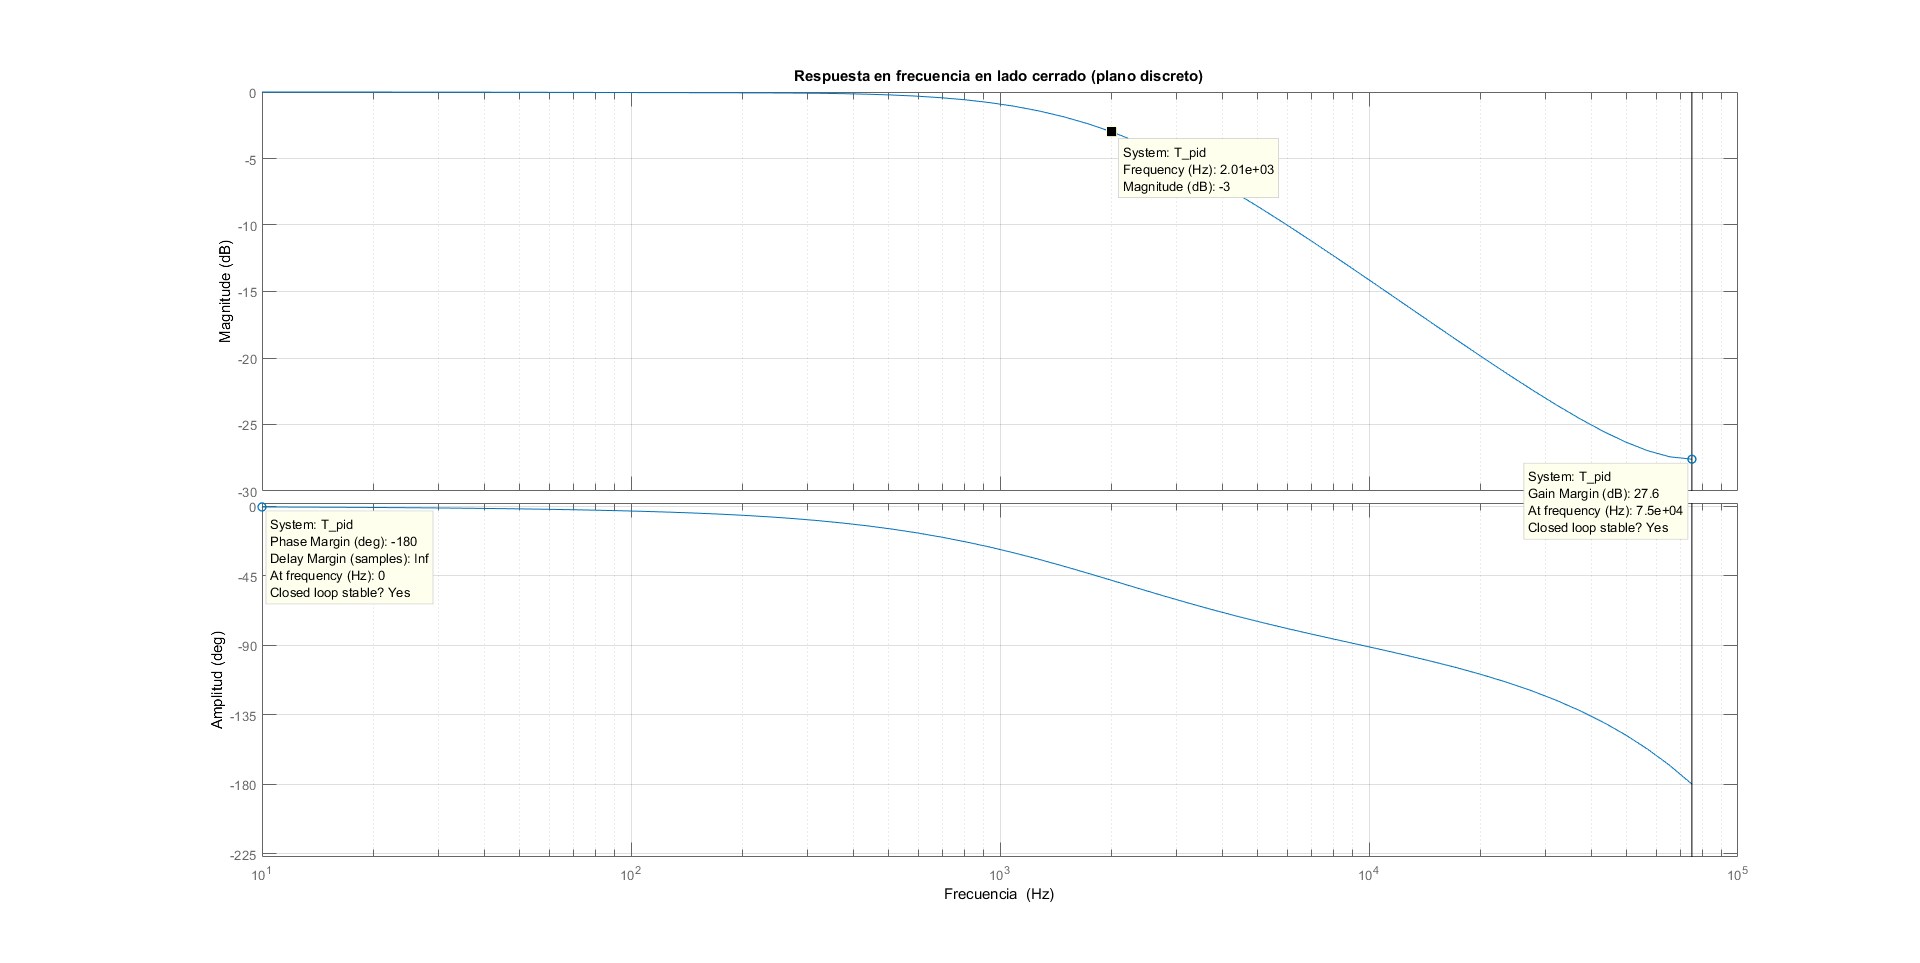
\includegraphics[width=\textwidth,height=\textheight,keepaspectratio]{buck_bode_discrete} 
		\caption{Respuesta en frecuencia - Diagrama de Bode - Sistema Discreto}
		\label{buck:bode_discrete}
	\end{sidewaysfigure}
	
	\begin{sidewaysfigure}
		\centering
		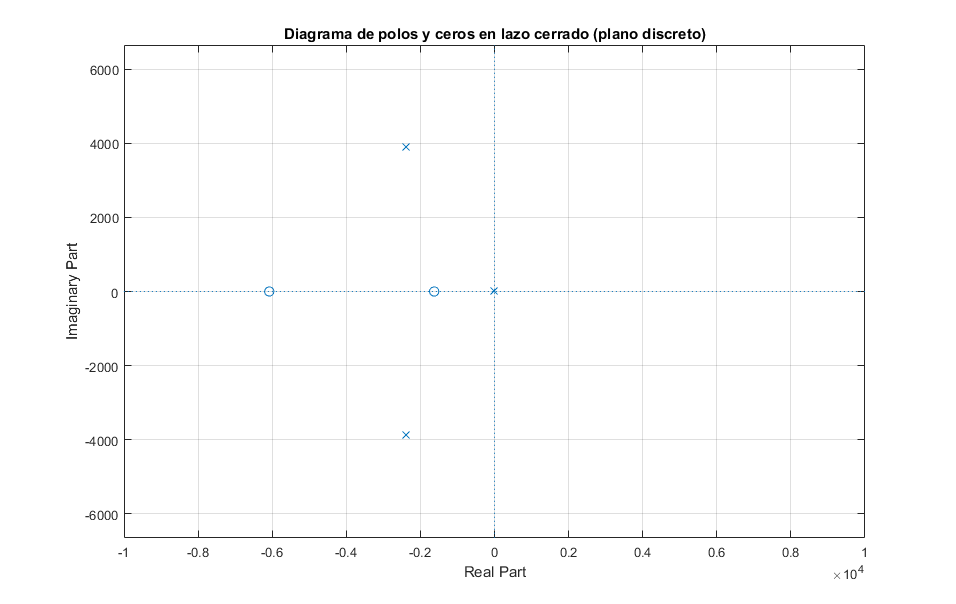
\includegraphics[width=\textwidth,height=\textheight,keepaspectratio]{buck_polos_ceros_discrete}
		\caption{Diagrama de polos y ceros - Sistema Discreto}
		\label{buck:polos_ceros_discrete}
	\end{sidewaysfigure}
	
	\begin{sidewaysfigure}
		\centering
		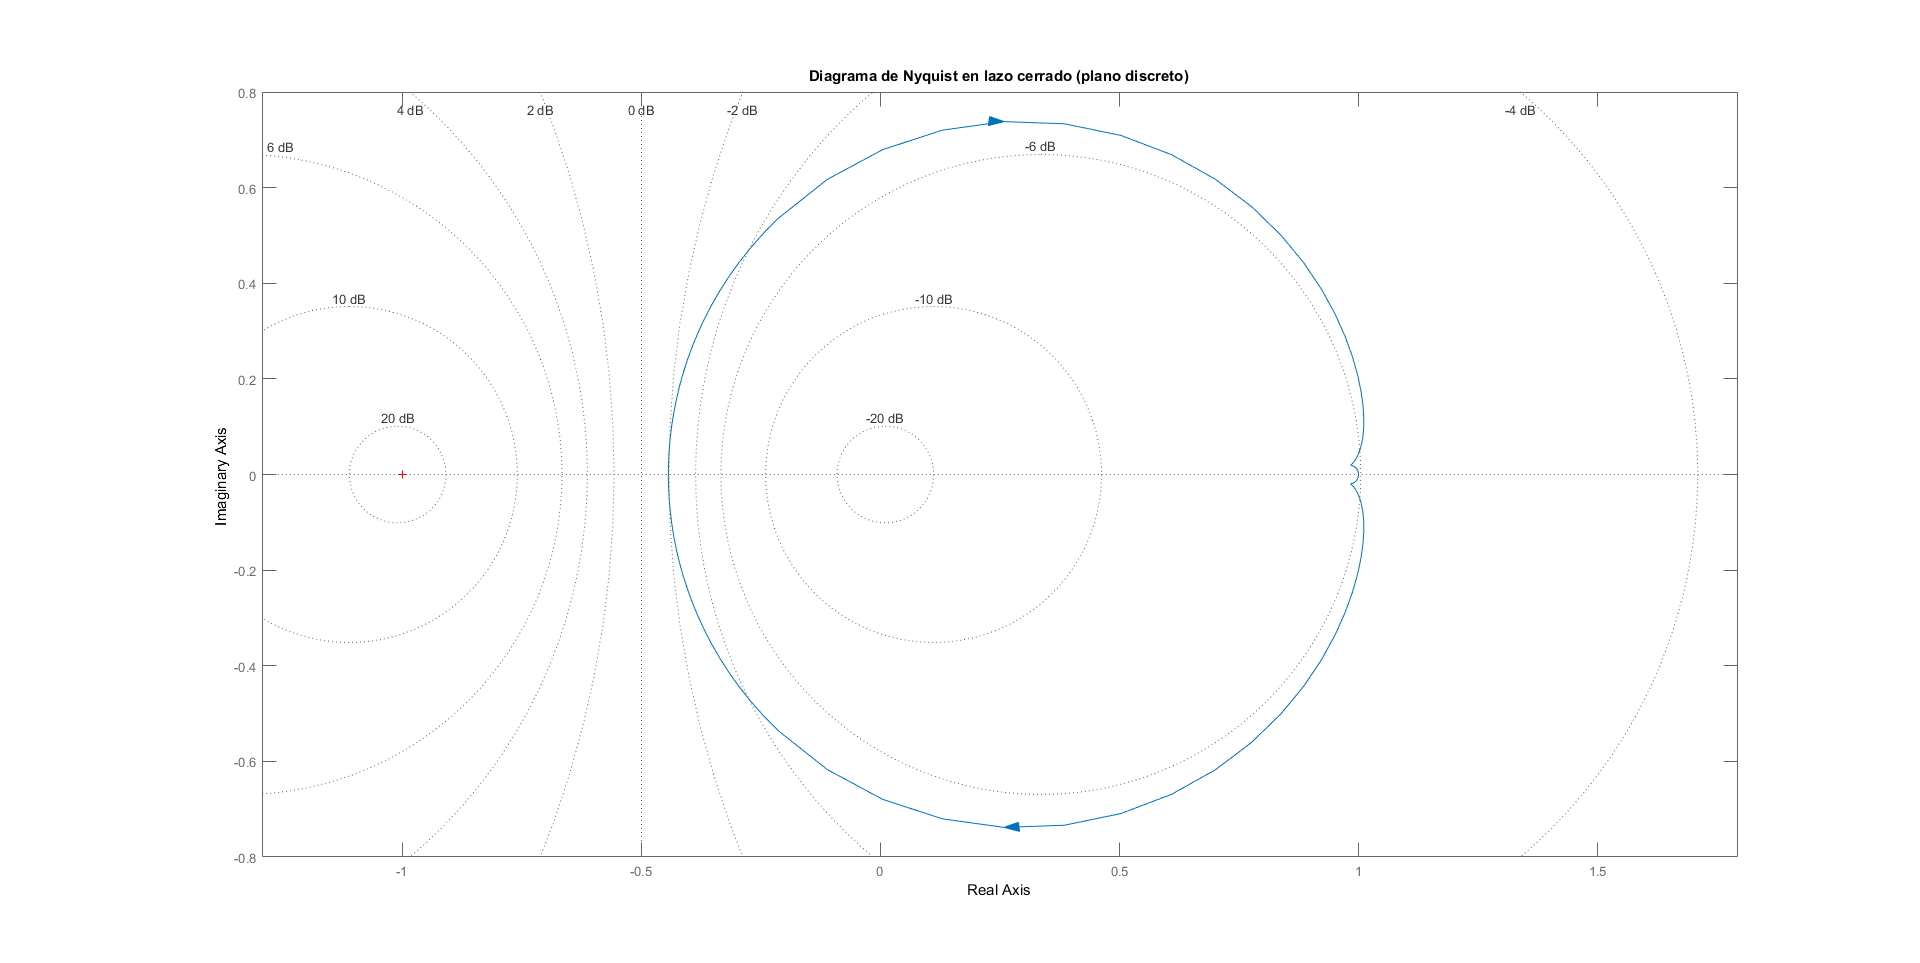
\includegraphics[width=\textwidth,height=\textheight,keepaspectratio]{buck_nyquist_discrete} 
		\caption{Diagrama de Nyquist - Sistema Discreto}
		\label{buck:nyquist_discrete}
	\end{sidewaysfigure}
	
\chapter{Circuito de control}

\section{Introducción}

El circuito de control es el encargado de controlar cada uno de los Convertidores Buck y aplicar el controlador PID además de monitorear las tensiones y corrientes de salida de los dos Buck y las salidas de tensión auxiliares de +5V y +3.3V. Las figuras \ref{control:main} y \ref{control:feedback} muestran los esquemáticos correspondientes. A continuación, vamos a analizar en detalle cada una de las partes que integran al circuito.

\begin{sidewaysfigure}
	\centering
	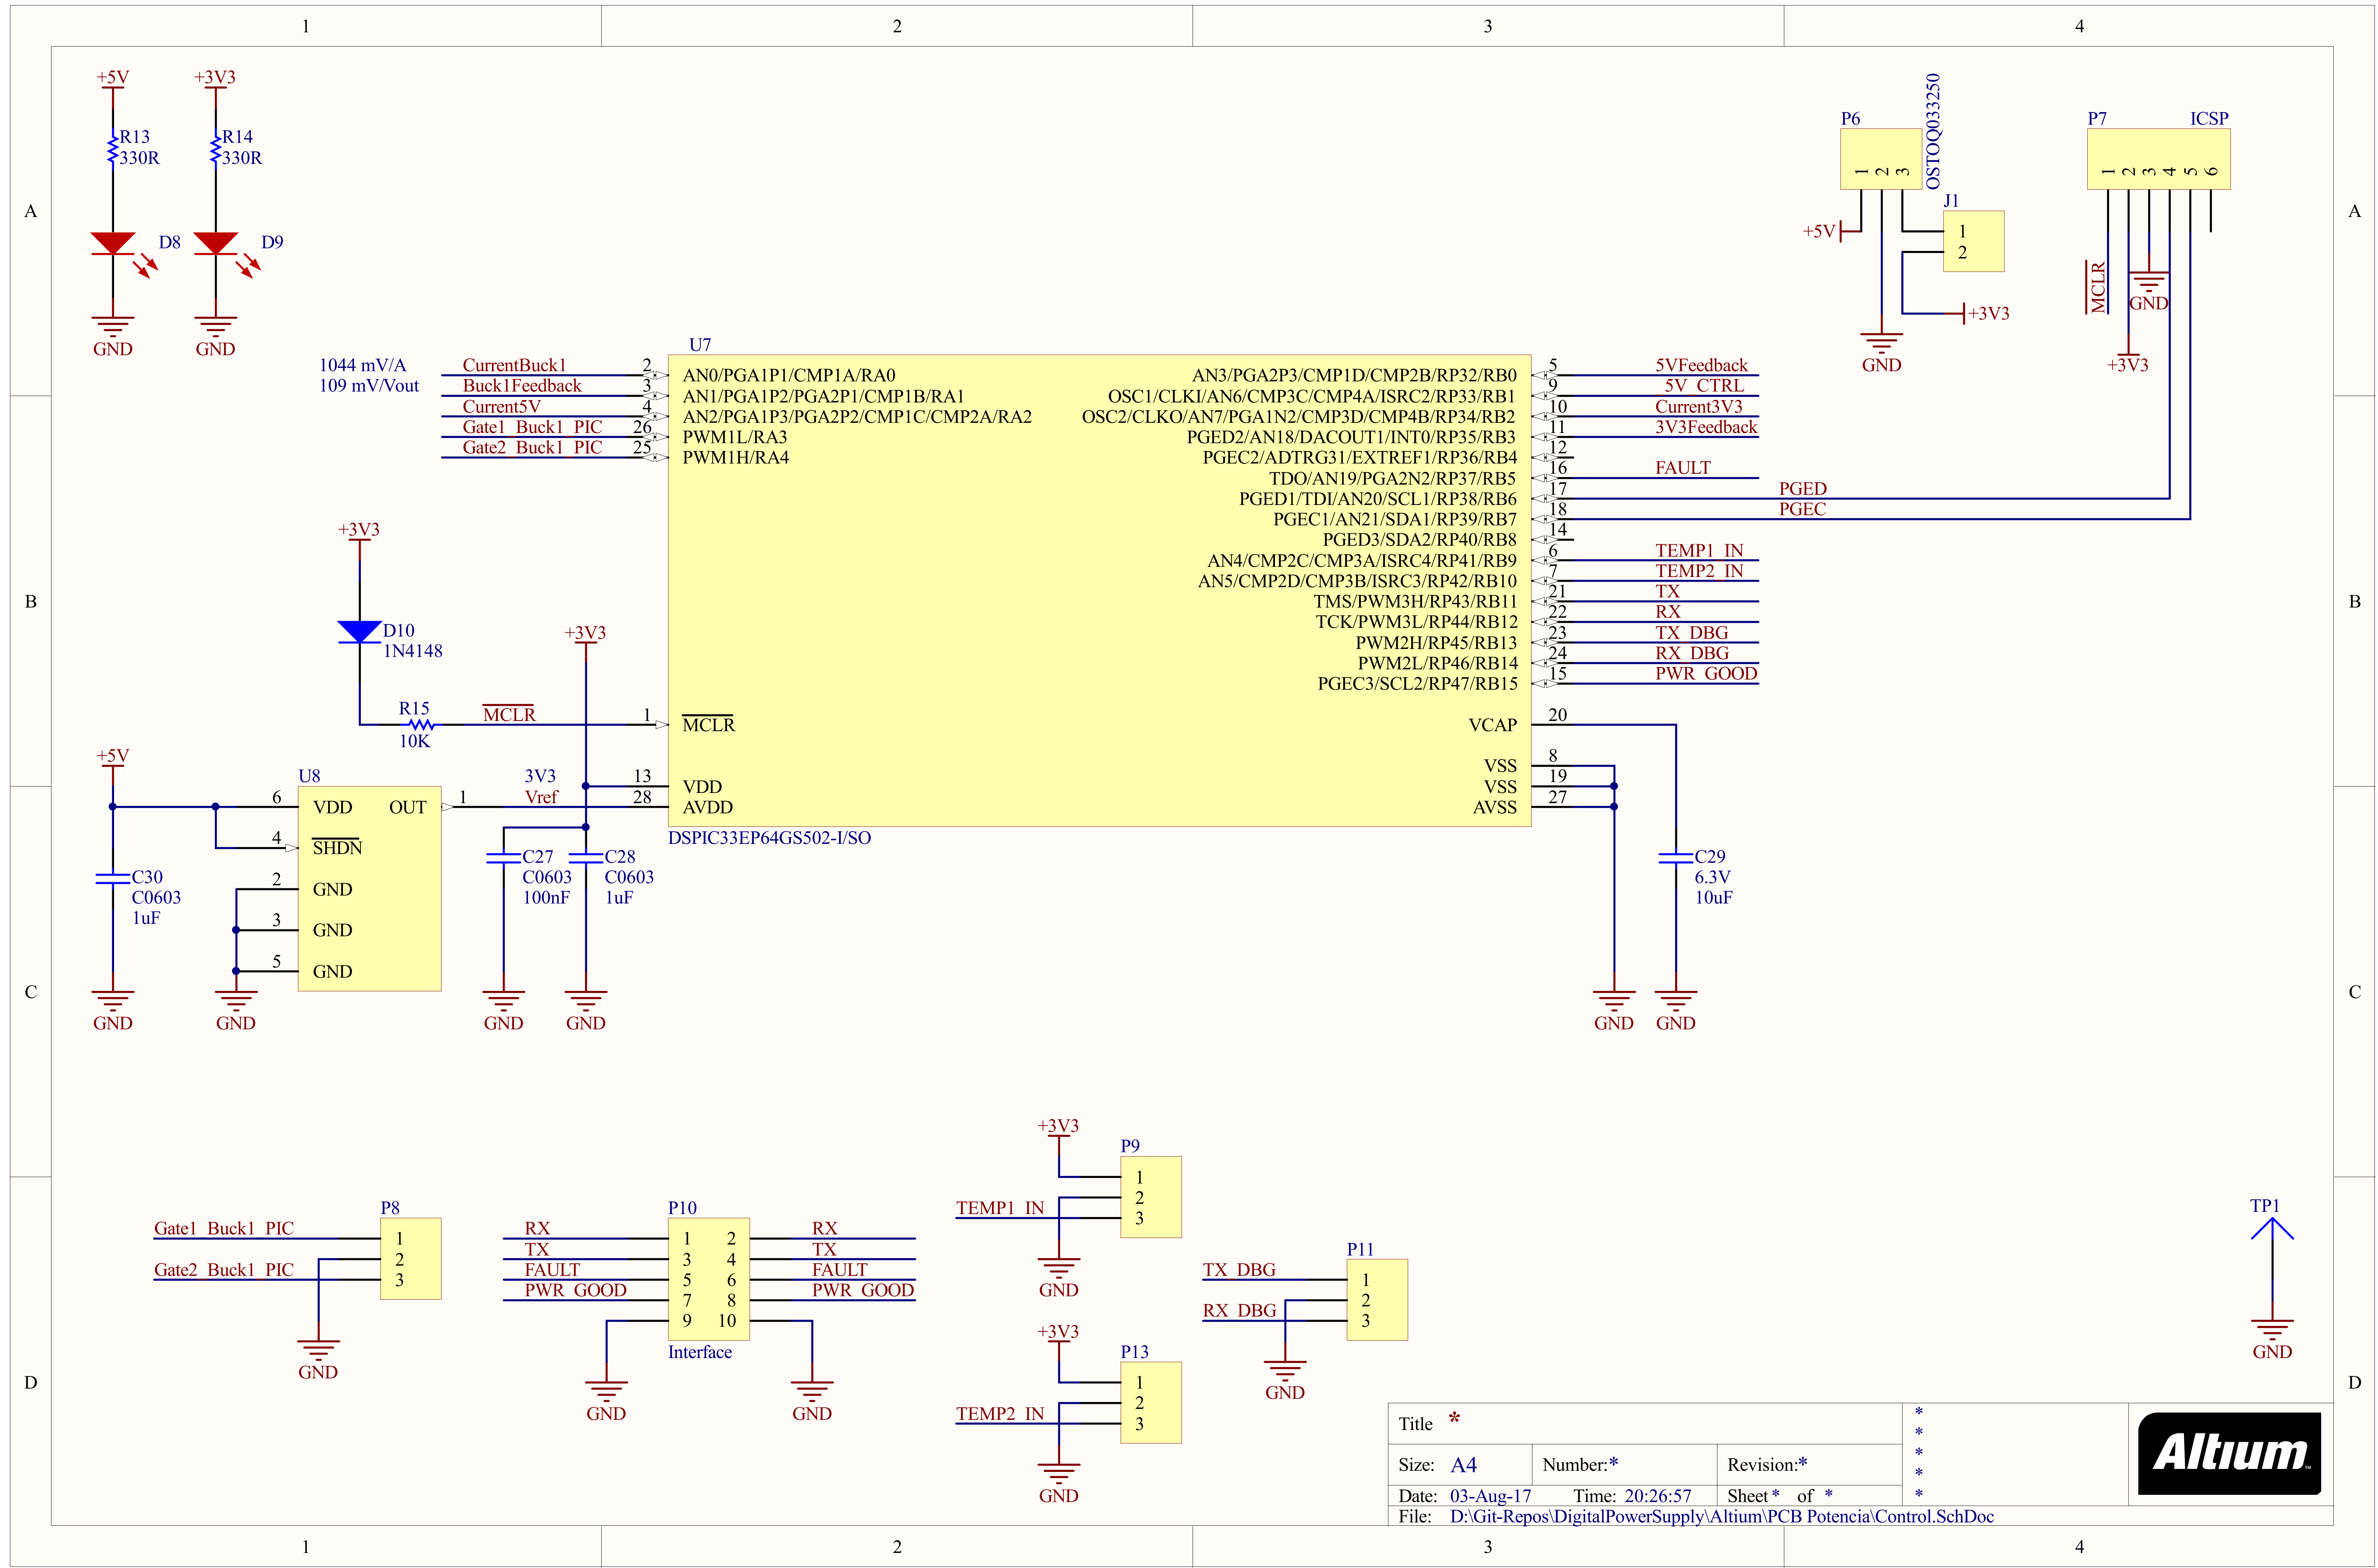
\includegraphics[width=\textwidth,height=\textheight,keepaspectratio]{sch_control_main} 
	\caption{Esquema principal del circuito de control}
	\label{control:main}
\end{sidewaysfigure}

\begin{sidewaysfigure}
	\centering
	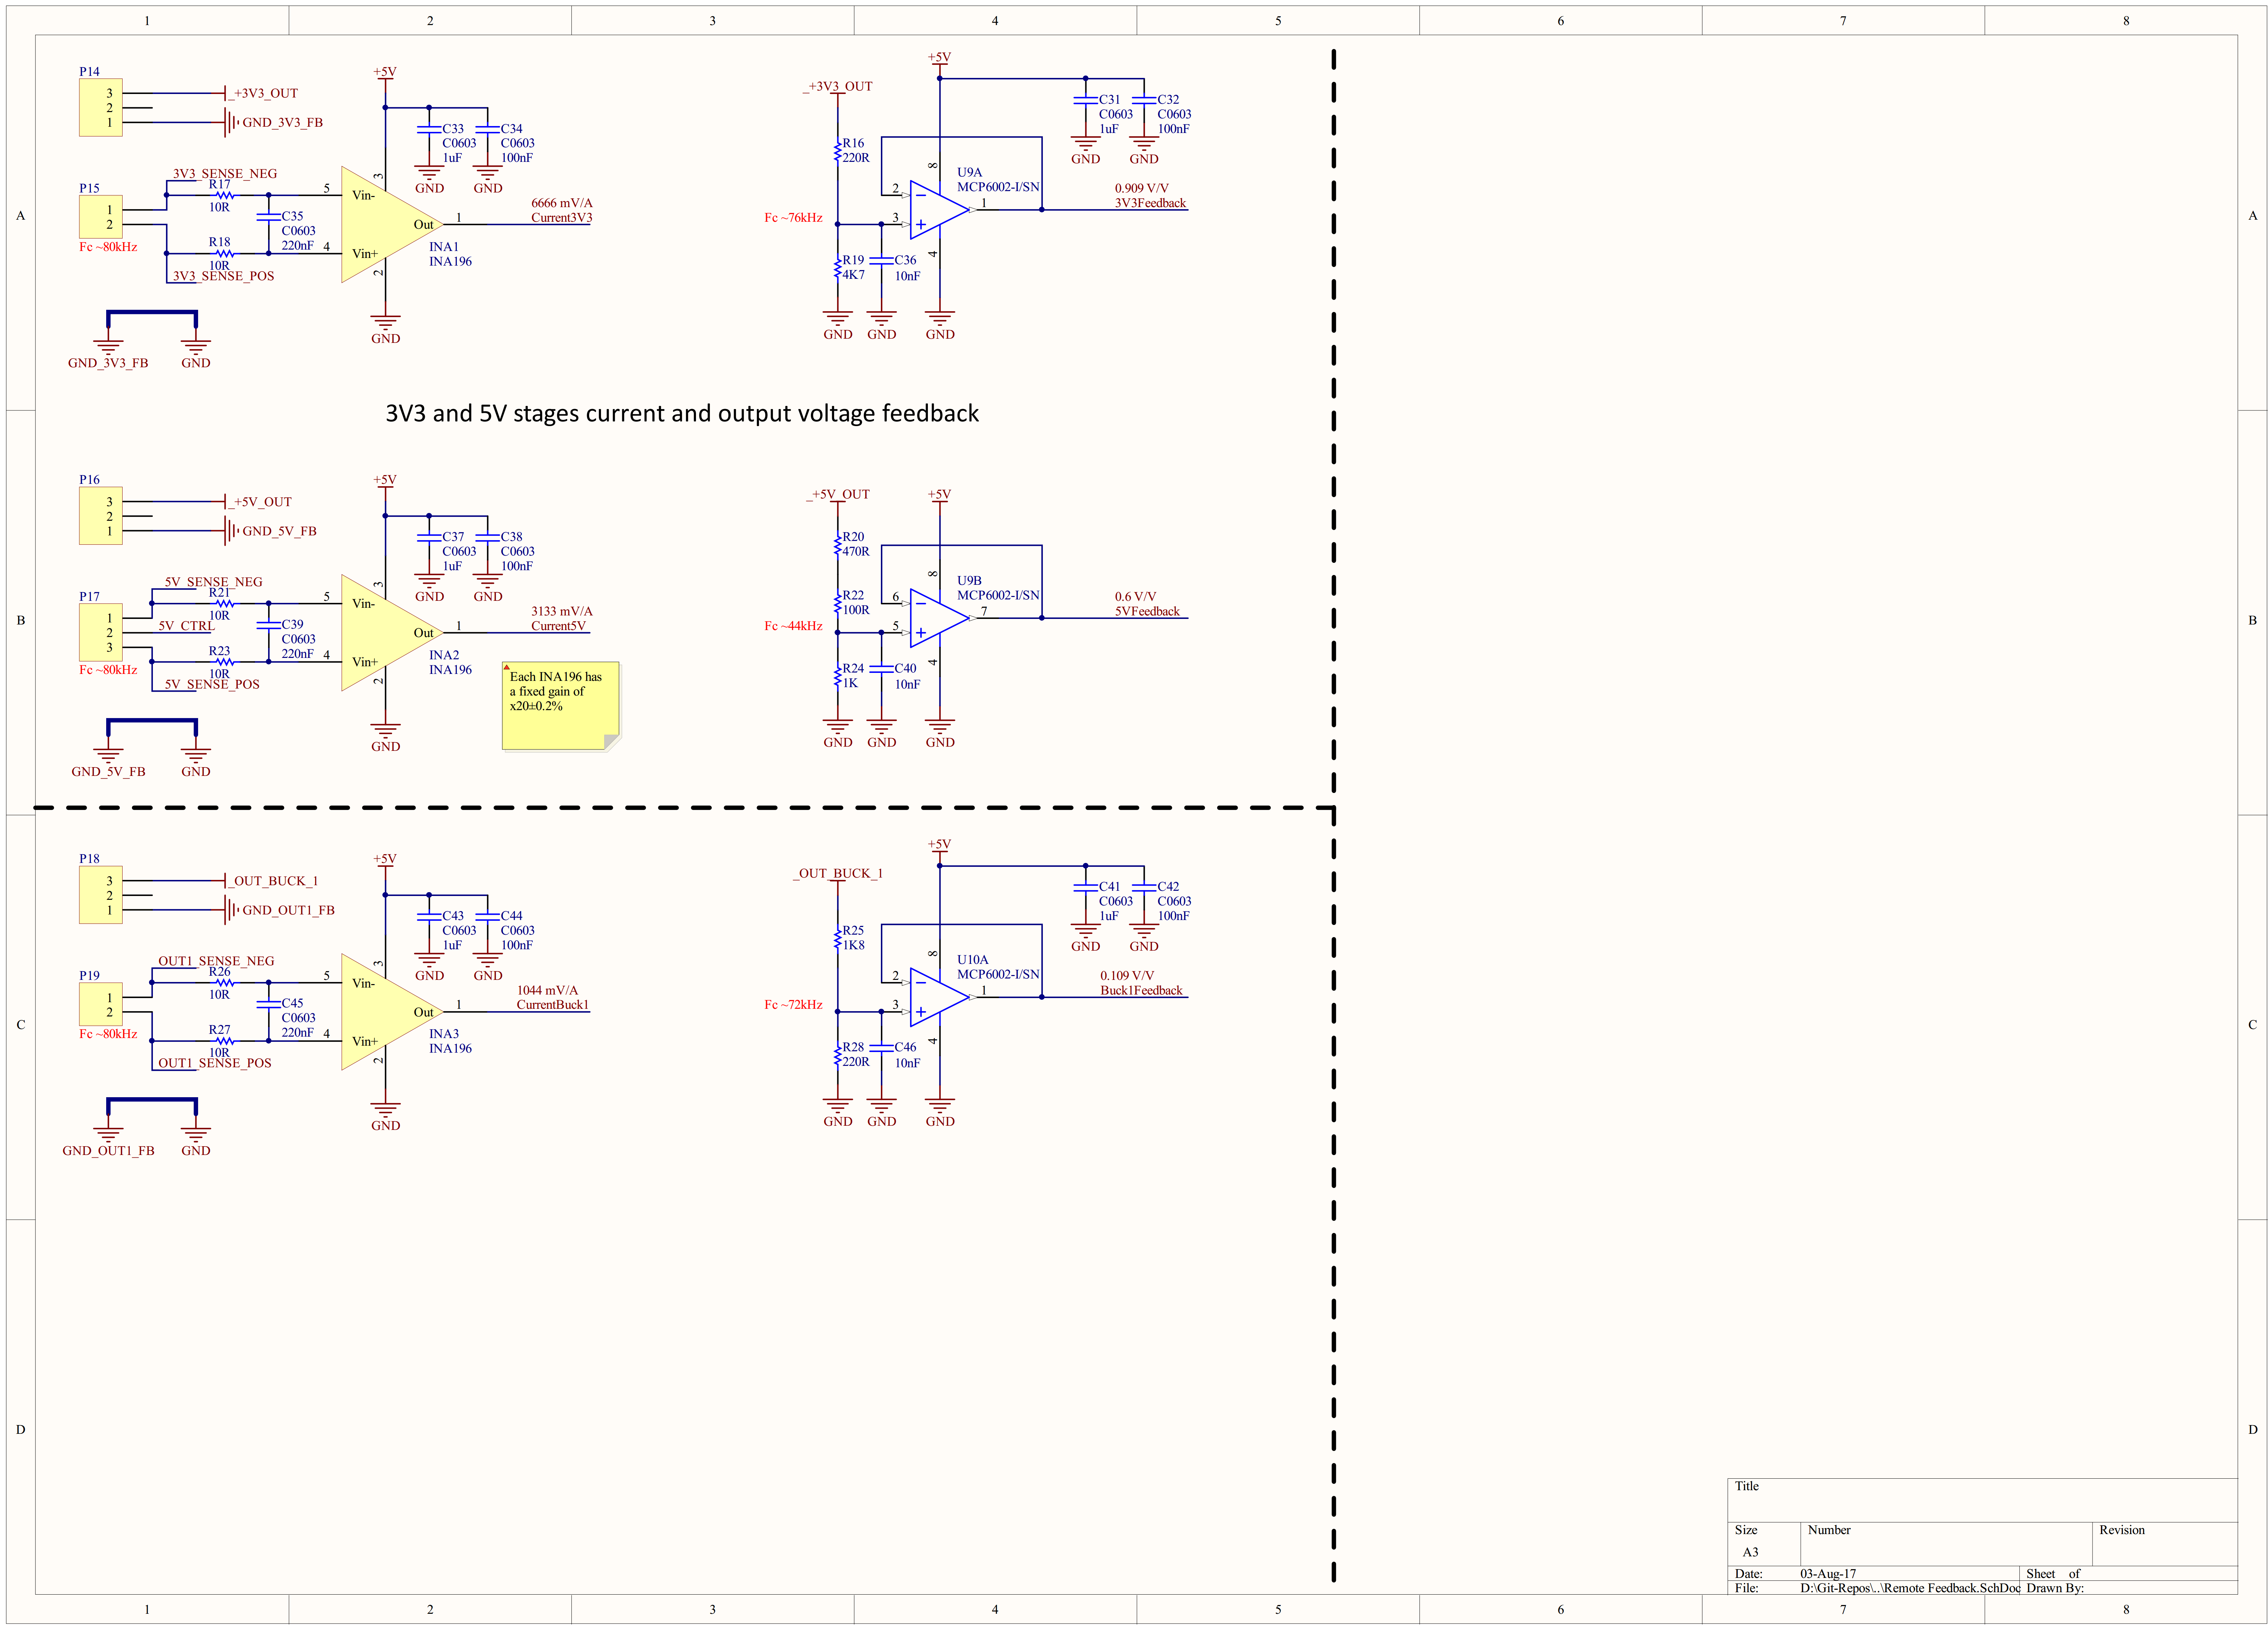
\includegraphics[width=\textwidth,height=\textheight,keepaspectratio]{sch_control_feedback} 
	\caption{Circuito de acondicionamiento de señal}
	\label{control:feedback}
\end{sidewaysfigure}

\section{Microcontrolador DSP}

El microcontrolador elegido es un dsPIC33FJ16GS402 de la empresa Microchip\textregistered capaz de trabajar a una velocidad de hasta 50 MIPS con 16KB de memoria FLASH y 2KB de memoria RAM. Las principales características por las que fue elegido son:

\begin{itemize}
	\item 50 MIPS de velocidad
	\item Módulo PWM de alta velocidad que permite un control preciso del Duty Cycle respecto a los convencionales
	\item Control de dead-time o tiempo muerto
	\item ADC de alta velocidad de 10 bits con circuitos Sample\&Hold dedicados lo que permite como tomar muestras de tensión y corriente de las salidas en forma simultánea sin ningún tipo de atraso entre una y otra
	\item Núcleo DSP con instrucciones MAC (multiply-accumulate) de ciclo único lo que permite la ejecución de algoritmos PID de forma rápida
\end{itemize} 

Como se explica arriba, este microcontrolador tiene la posibilidad de generar tiempos muertos o Dead-Time en las señales PWM para los Convertidores Buck. Como recordamos, los Buck implementados son del tipo sincrónico por lo que mientras un MOSFET se enciende el otro permanece apagado. Debido a que el tiempo de transición entre encendido y apagado no es instantáneo es necesario introducir un tiempo muerto entre ambos estados en donde ambos MOSFET se encuentran apagados. En la imagen \ref{deadtime} se ilustra el comportamiento descrito.

\begin{figure}[H]
	\centering
	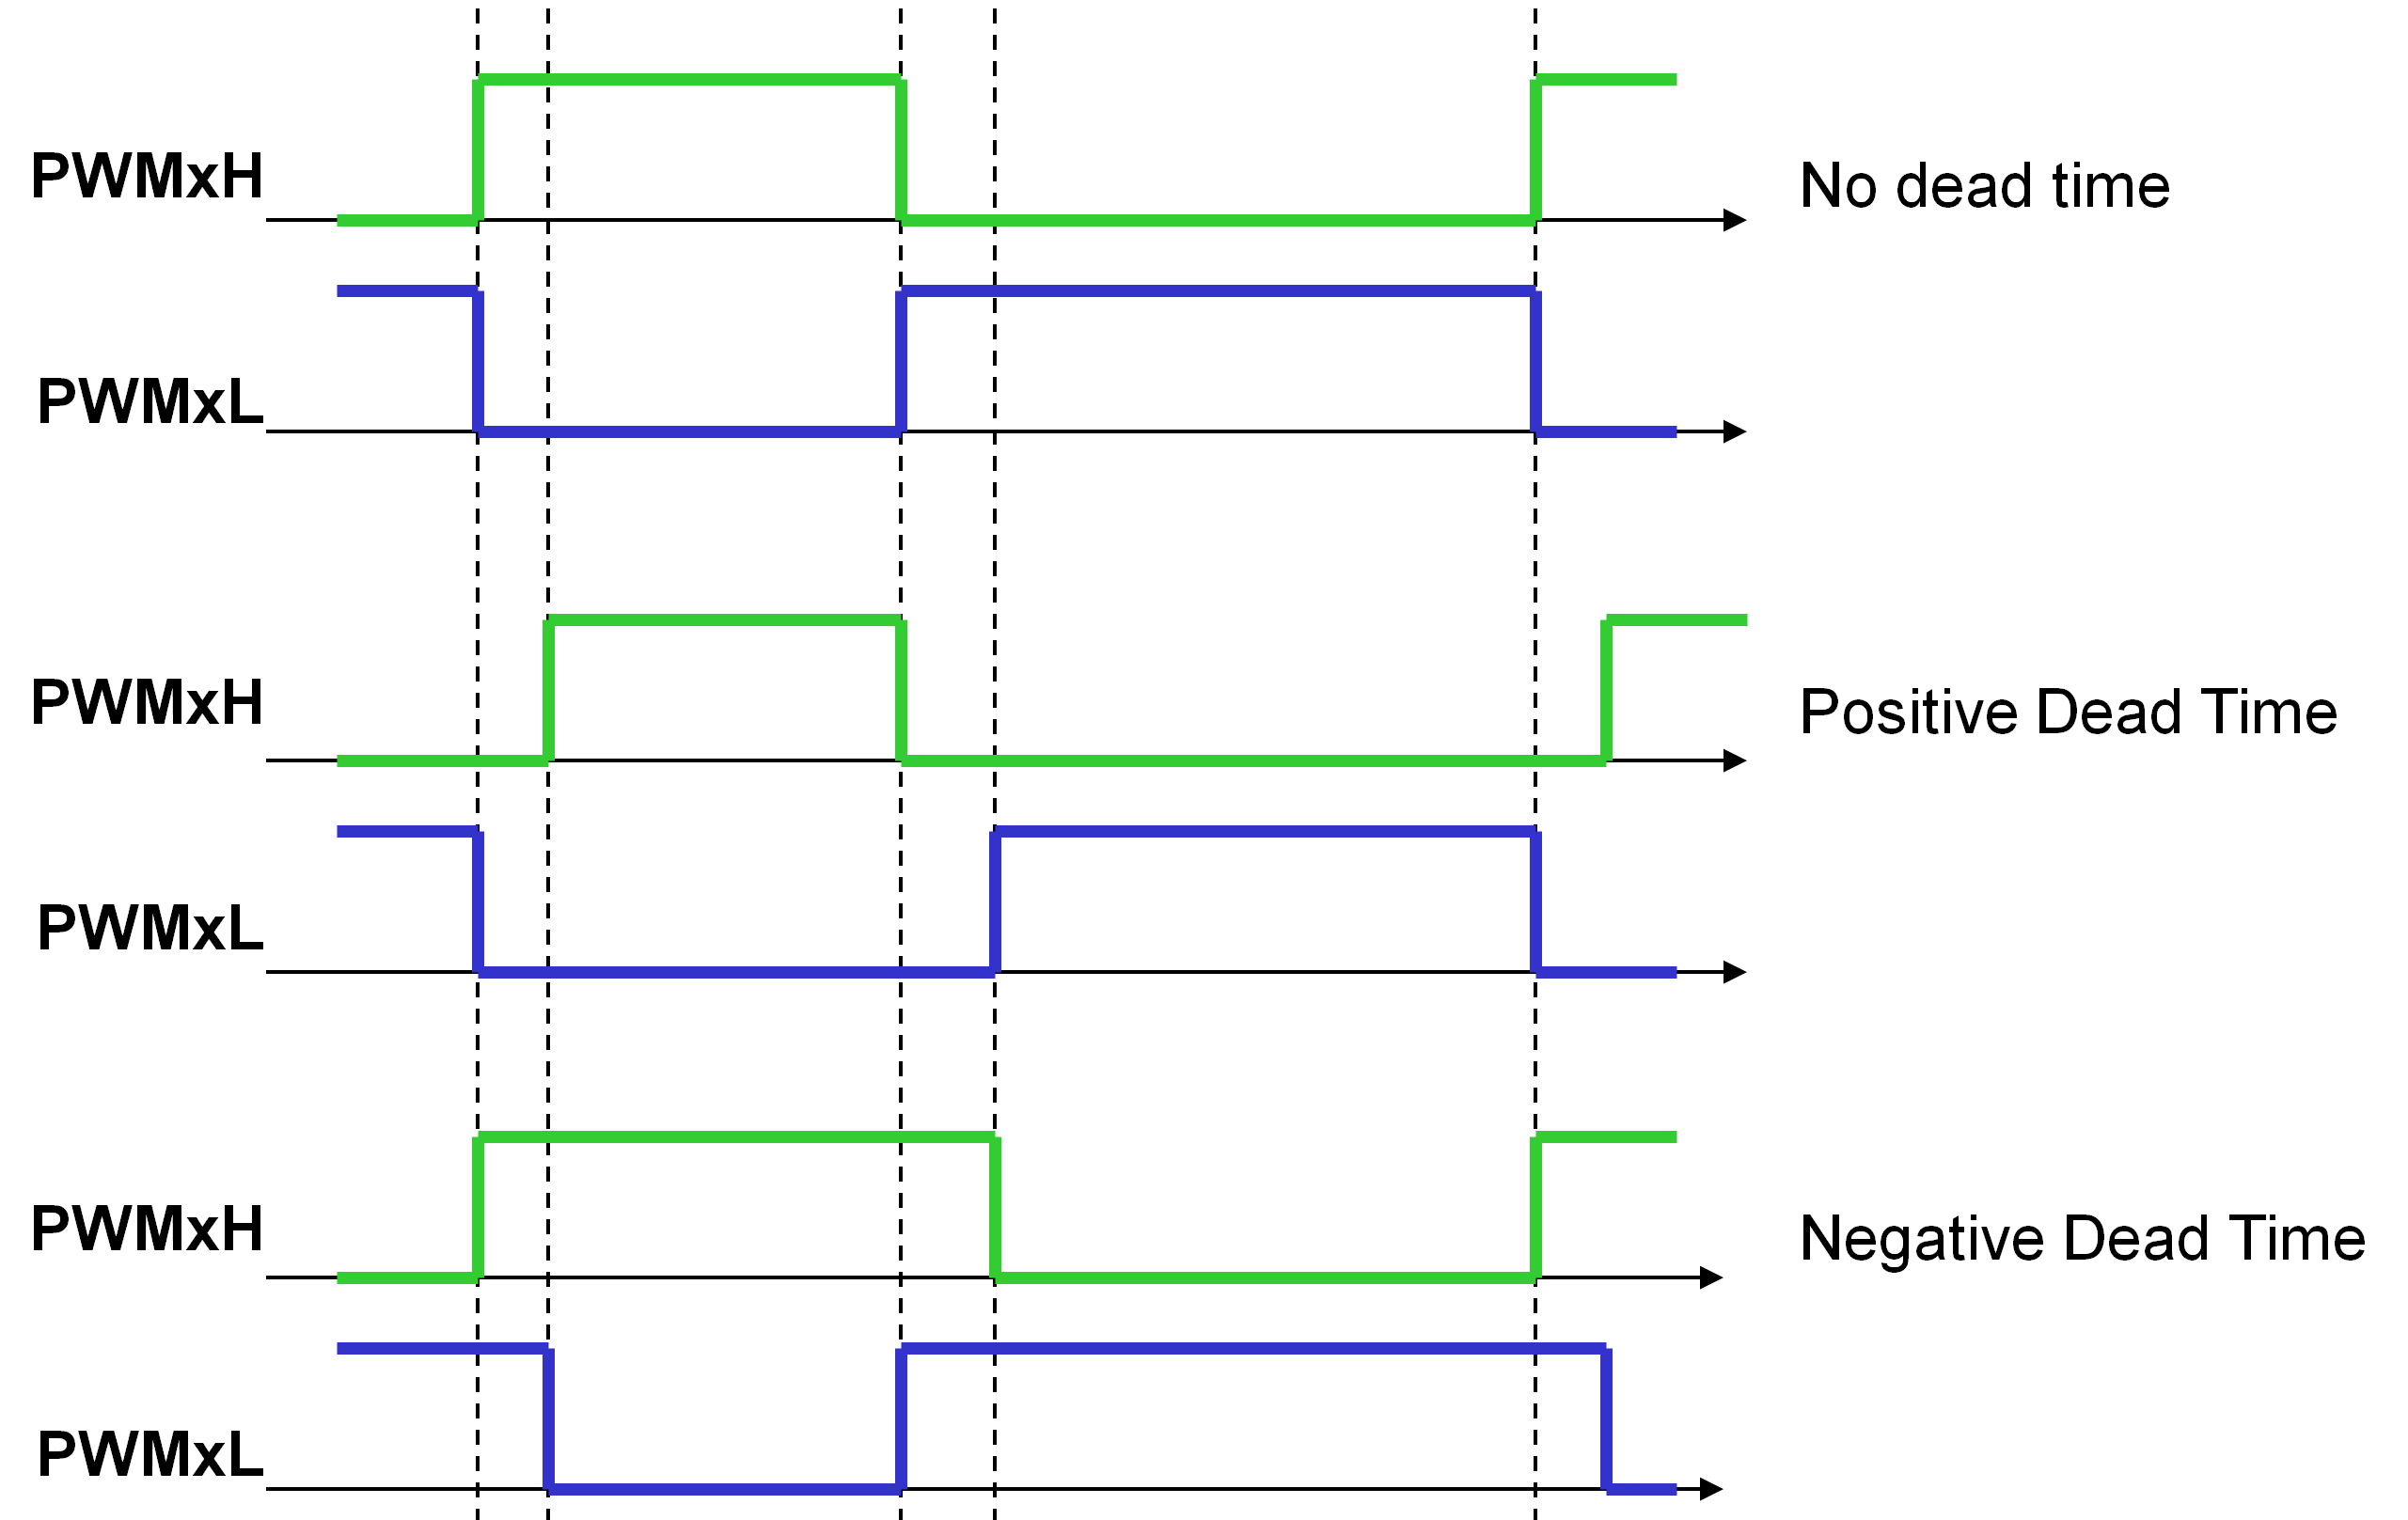
\includegraphics[width=0.9\textwidth,height=\textheight,keepaspectratio]{deadtime}
	\caption{Ilustración del concepto de Dead-Time o tiempo muerto}
	\label{deadtime}
\end{figure}

\section{Metodología de muestreo}

El módulo ADC que tenemos disponible contiene más de un circuito Sample\&Hold, disponemos de 3 Sample\&Hold dedicados y uno compartido:

\begin{figure}[H]
	\centering
	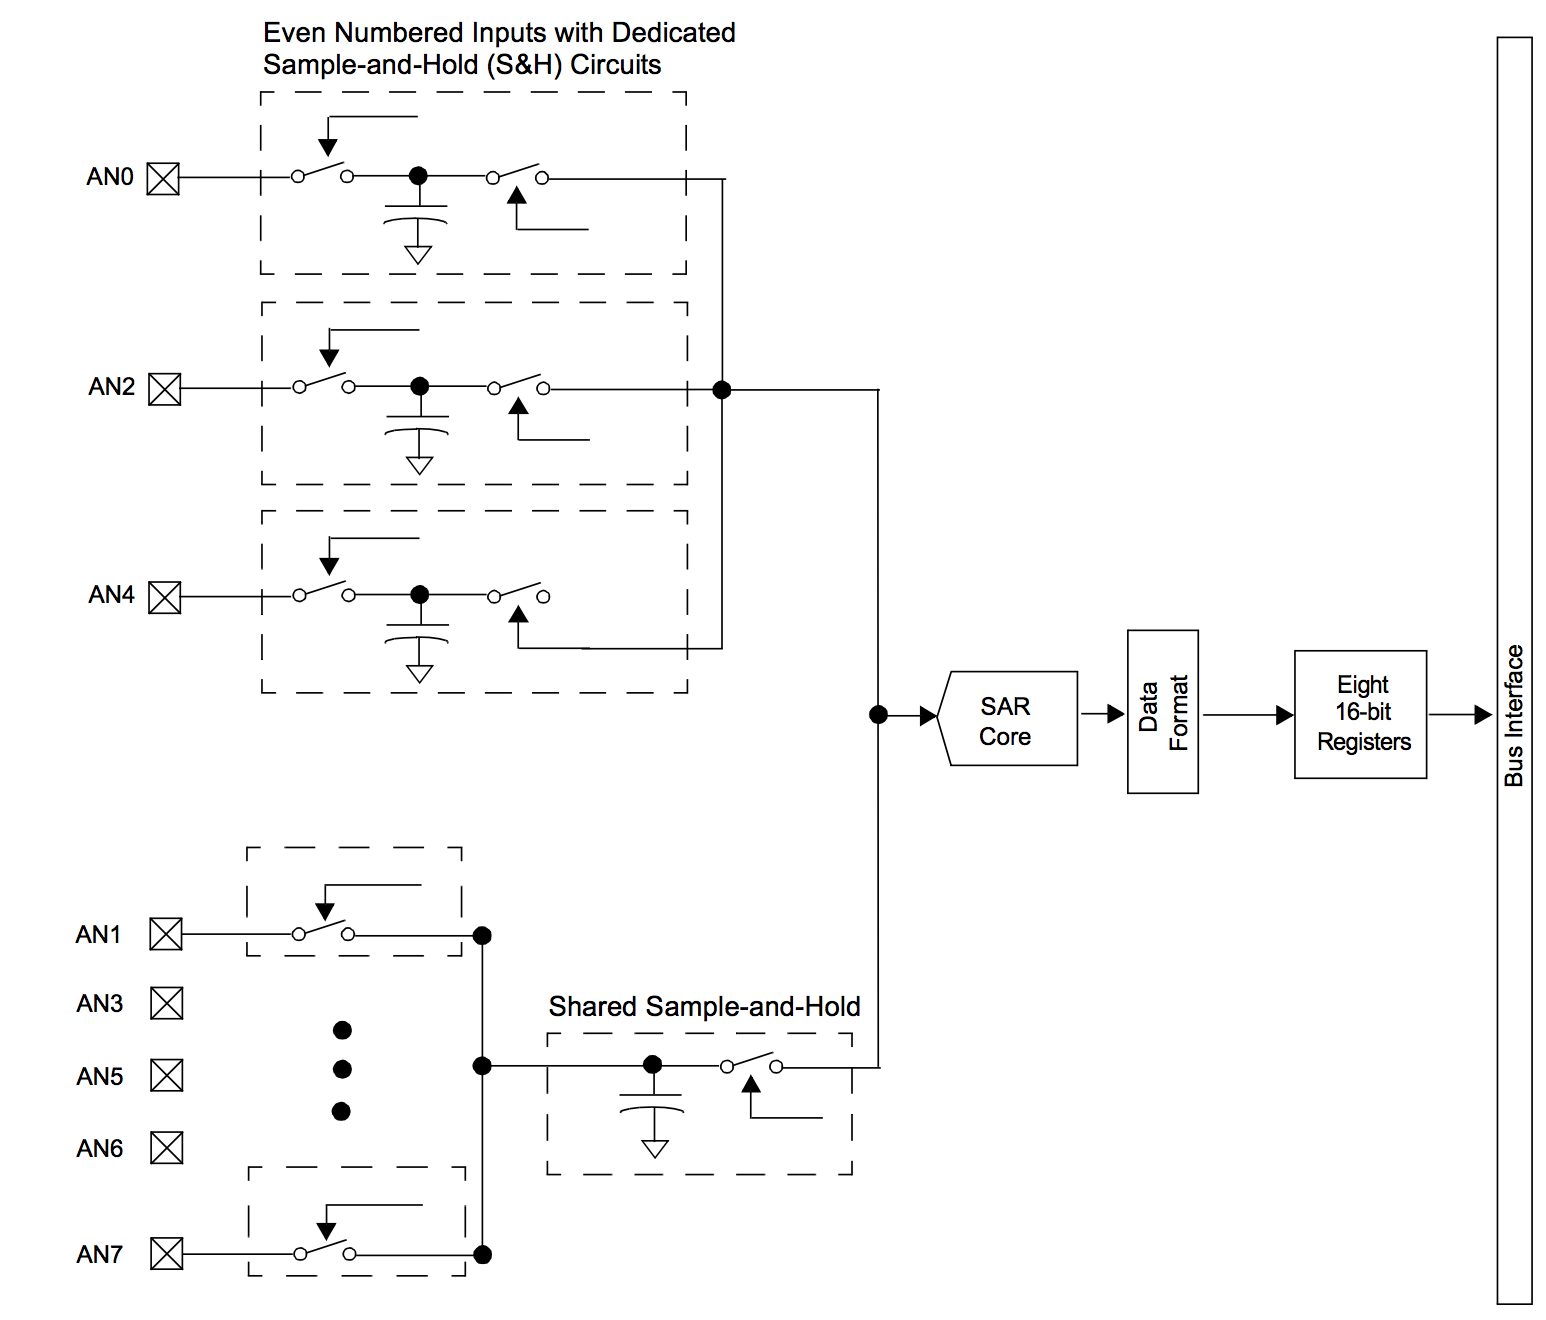
\includegraphics[width=0.7\textwidth,height=\textheight,keepaspectratio]{sh_diagram}
	\caption{Estructura del módulo ADC}
\end{figure}
	
El sistema funciona de a pares, es decir, cada vez que se inicia una conversión un par de entrada analógicas son capturadas. Esto nos permite medir en un mismo instante de tiempo la tensión y la corriente de salida, sin embargo, solo disponemos de un SAR por lo que solo se convierte un canal a la vez. Existen varias configuraciones sobre el orden de muestreo y conversión del módulo, el siguiente fue el elegido:

\begin{enumerate}
	\item Se inicia el pedido de inicio de muestreo del par. Esto iniciará el muestreo de una entrada par y su impar asociada, por ejemplo, AN0 y AN1, AN2 y AN3, etcétera.
	\item Luego de pasado el tiempo de sincronismo ambos canales (par e impar) muestrean de forma simultánea.
	\item Una vez terminado el muestreo se inicia la conversión del canal par.
	\item Finalmente, terminada la conversión del canal par, se inicia la conversión del canal impar de forma automática, que luego de haberse finalizado su conversión se genera una interrupción y termina así el proceso.
\end{enumerate}

\begin{figure}[H]
	\centering
	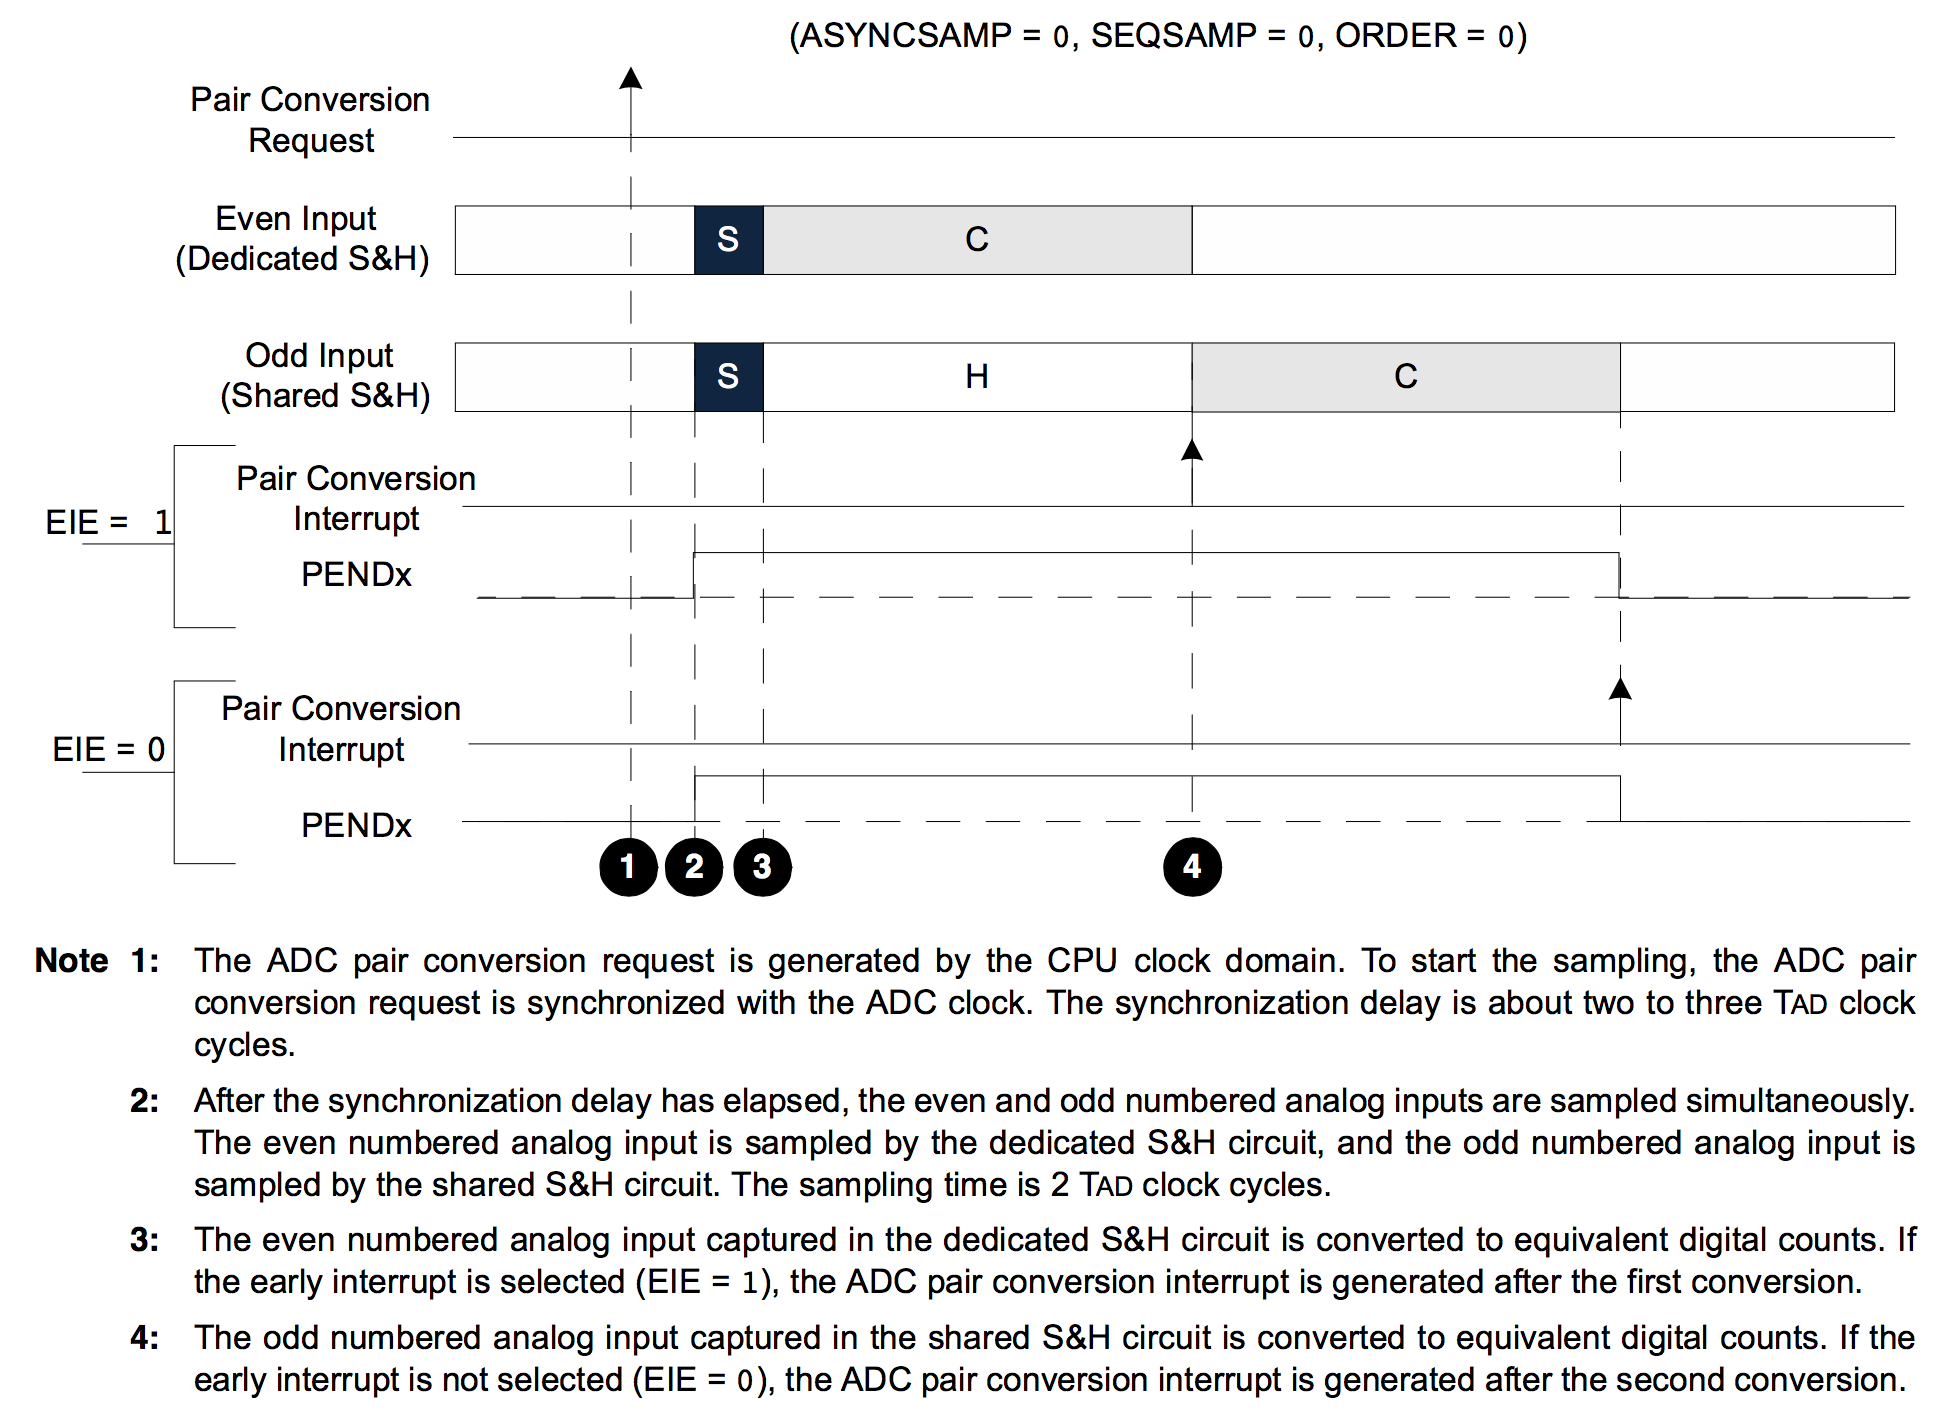
\includegraphics[width=\textwidth,height=\textheight,keepaspectratio]{adc_conversion}
	\caption{Proceso de muestreo y conversión}
\end{figure}

Este proceso se raliza para ambos buck de forma intercalada aprovechando así al máximo el uso del procesador:

\begin{figure}[H]
	\centering
	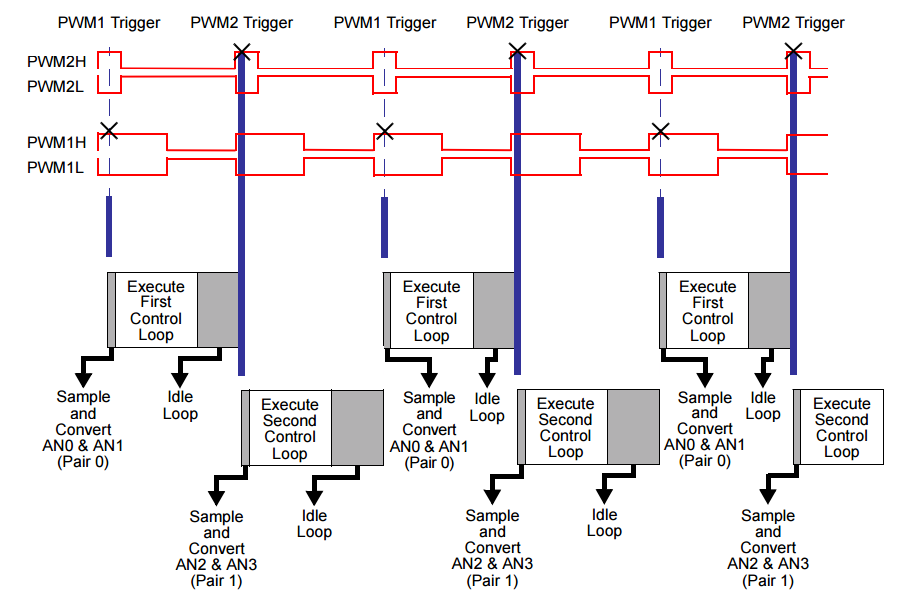
\includegraphics[width=\textwidth,height=\textheight,keepaspectratio]{cpu-load}
	\caption{Intercalado del muestreo para los Convertidores Buck}
\end{figure}


\section{Leading-Edge Blanking}

Para la correcta lectura de la tensión de salida se utiliza una funcionalidad llamada Leading-Edge Blanking que provee el módulo PWM del DSP. Básicamente permite que la captura del ADC se realize un determinado tiempo después de los flancos de PWM para de este modo no capturar el ruido de conmutación y obtener una lectura erronea:

\begin{figure}[H]
	\centering
	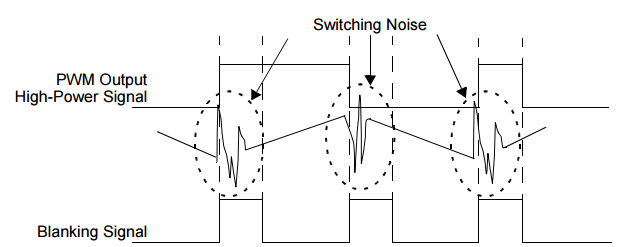
\includegraphics[width=\textwidth,height=\textheight,keepaspectratio]{leading-edge-blanking}
	\caption{Leading-Edge Blanking}
\end{figure}


\section{Acondicionamiento de las tensiones de salida} \label{acondicionamiento-tensiones}

El siguiente es el circuito de realimentación de tensión usado para poder tomar las tensiones de los dos convertidores Buck y las salidas auxiliares de +5V y +3.3V.

\begin{figure}[H]
	\centering
	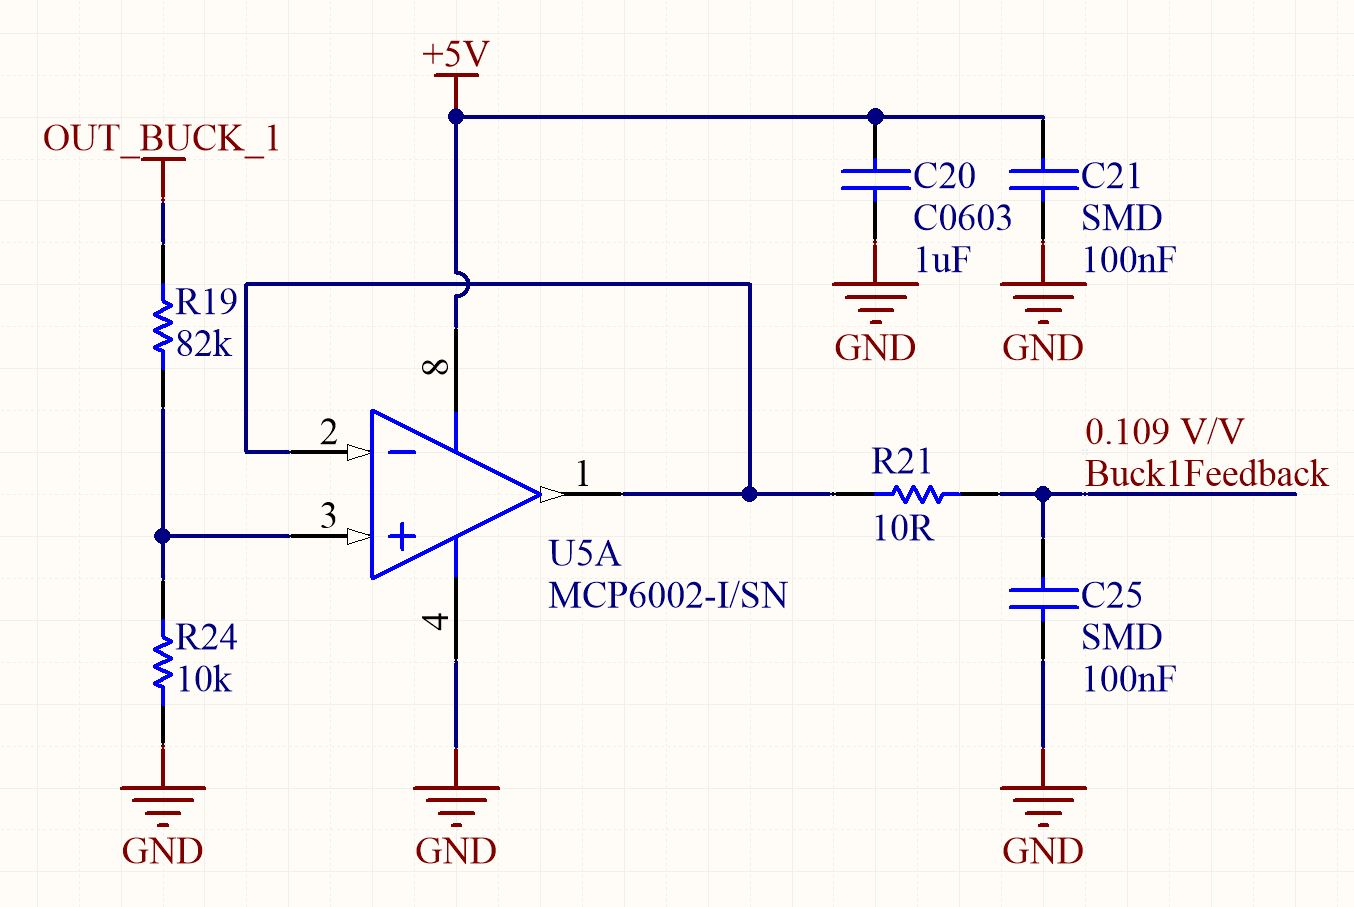
\includegraphics[width=\textwidth,height=\textheight,keepaspectratio]{voltage_feedback}
	\caption{Circuito de realimentación de tensión}
	\label{voltage_feedback_circuit}
\end{figure}

El circuito es el mismo para todas las salidas variando únicamente el divisor resistivo de entrada al seguidor de tensión. A la salida del operacional se implementó un simple filtro pasa-bajos con una frecuencia de corte de 160kHz para eliminar los ruidos de alta frecuencia que puedan generarse como consecuencia de la conmutación. 

Según el datasheet de nuestro microcontrolador, la resolución efectiva del ADC es de 9.4 bits y teniendo una tensión de referencia para el mismo de 3.3V con una variación máxima de $\pm2.5\%$, podemos calcular la resolución de tensión que tenemos al medir cada una de las salidas de la fuente y el error asociado.

La resolución en tensión del ADC puede ser calculada como:

\begin{equation}
	Res = 3.3V / 2^{9.4} = 4.88 mV
\end{equation}

Vamos a calcular el factor de atenuación de cada salida que viene dado por el valor de las resistencias en el divisor de tensión, tomando como ejemplo el circuito de la figura \ref{voltage_feedback_circuit} el factor de atenuación esta dado como:

\begin{equation}
	Vo/Vi = \frac{10}{10 + 82} = 0.109
\end{equation}

Con la resolución del ADC y el factor de atenuación podemos calcular entonces la resolución que tenemos al medir la tensión de salida del Buck 1 en este caso:

\begin{equation}
	Resolucion \ salida = \frac{Res}{Vo/Vi} = \frac{\num{4.88e-3} mV}{0.109} = 45 mV
\end{equation}

Como la tensión de referencia tiene una variación de $\pm2.5\%$, la lectura del ADC se ve directamente afectada por esta referencia, por lo que la resolución de la tensión de salida también tendrá un error del $\pm2.5\%$ que se traduce en una variación de $\pm1.2mV$. En la siguiente tabla se muestran los resultados del mismo procedimiento aplicado a las demás salidas:

\begin{table}[H]
	\centering
	\begin{tabular}{M{2cm}M{5cm}M{3cm}M{3cm}} \toprule
		Parámetro & Factor de atenuación Vo/Vi & Resolución & Error 
		\\ \midrule
		$V_{buck1}$ & 0.109 & 45mV & $\pm1mV$ \\
		$V_{buck2}$ & 0.109 & 45mV & $\pm1mV$ \\
		$V_{5V}$ & 0.641 & 7.61mV & $\pm0.2mV$ \\
		$V_{3.3V}$ & 0.909 & 5.37mV & $\pm0.13mV$ \\
		\bottomrule
	\end{tabular}
	\caption{Resolucíon de las tensiones de salida}
\end{table}

\section{Acondicionamiento de las corrientes de salida}

\begin{figure}[H]
	\centering
	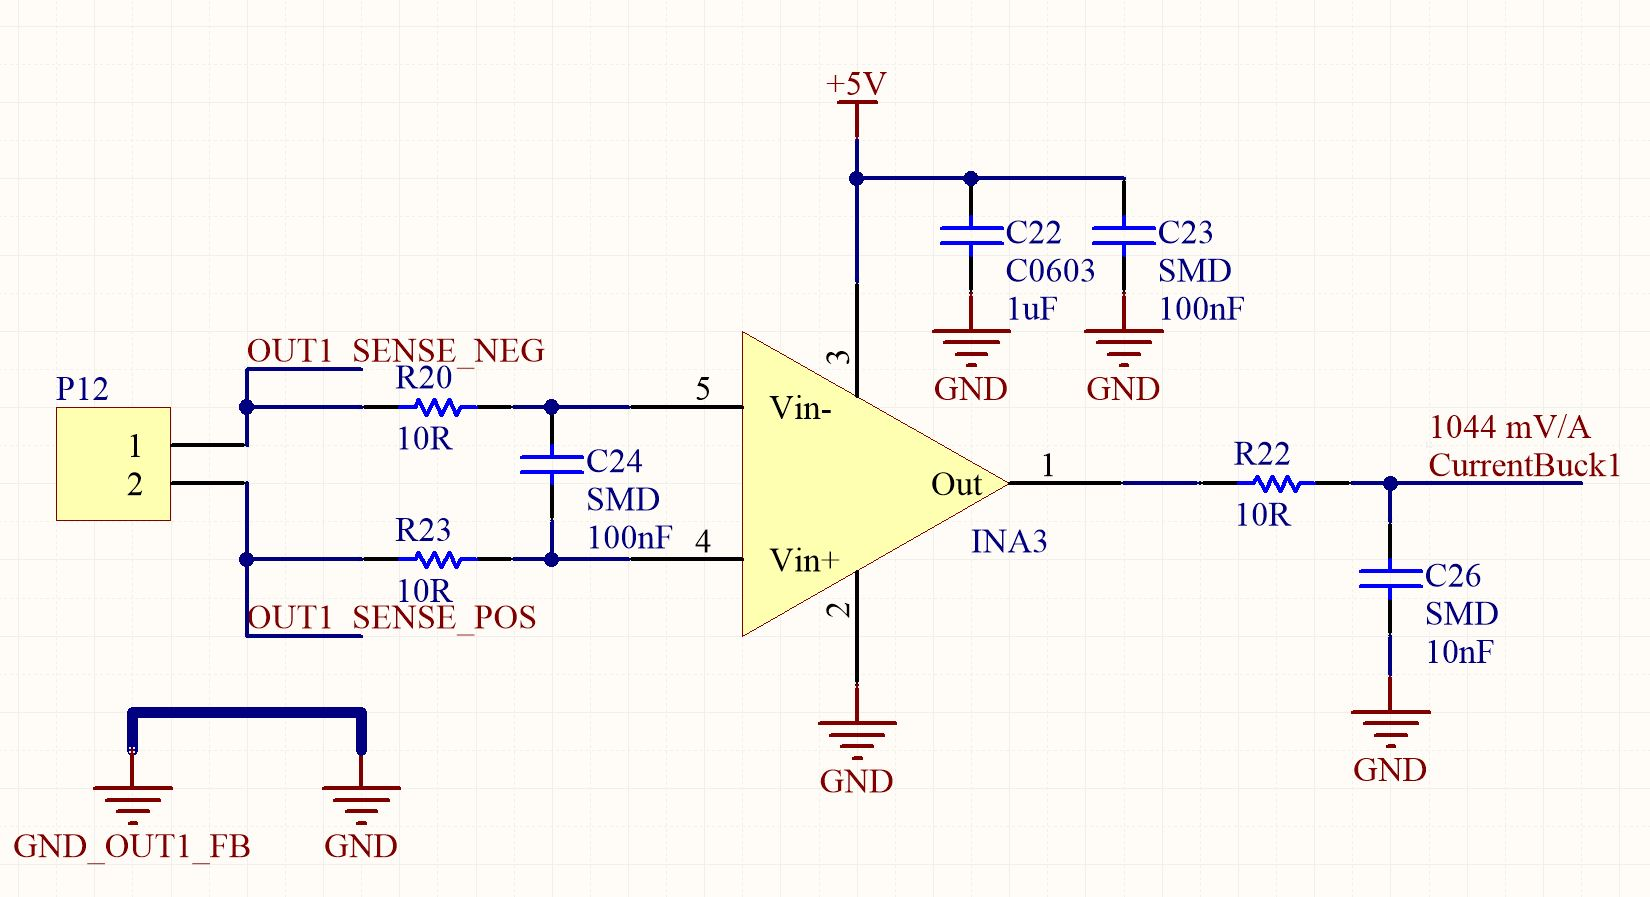
\includegraphics[width=\textwidth,height=\textheight,keepaspectratio]{current_feedback}
	\caption{Circuito de realimentación de corriente}
\end{figure}

Para medir la corriente de salida se toma la señal diferencial proveniente de las resistencias ubicadas en cada salida y se conectan a un amplificador para sensado de corriente INA196 pasando primero por un filtro pasa-bajos en la entrada. El amplificador tiene una ganancia fija de 20 por lo que las resistencias de sensado se calcularon en base a esta ganancia para obtener una tensión máxima de 3.3V a la salida. El circuito es el mismo para todas las salidas.

Utilizando la resolución del ADC obtenida en la sección anterior podemos calcular la resolución de corriente que tenemos en cada salida. Como tenemos una ganancia de 20 la resolución de tensión del ADC pasa a ser de:

\begin{equation}
	Res = 4.88mV / 20 = 244\mu V
\end{equation}

Tomemos como ejemplo la salida del Buck 1 cuya resistencia de sensado es de $52.2m\Omega$:

\begin{equation}
	Resolucion \ Corriente = Res / 52.2m\Omega = 4.67mA
\end{equation}

Aplicando el mismo proceso a todas las demás salidas:

\begin{table}[H]
	\centering
	\begin{tabular}{M{2cm}M{5cm}M{3cm}M{3cm}} \toprule
		Parámetro & Resistencia de sensado & Resolución & Error 
		\\ \midrule
		$I_{buck1}$ & $52.2m\Omega$ & 4.67mA & $\pm0.11mA$ \\
		$I_{buck2}$ & $52.2m\Omega$ & 4.67mA & $\pm0.11mA$ \\
		$I_{5V}$ & $157m\Omega$ & 1.55mA & $\pm0.04mA$ \\
		$I_{3.3V}$ & $500m\Omega$ & 0.48mA & $\pm0.01mA$ \\
		\bottomrule
	\end{tabular}
	\caption{Resolucíon de las corrientes de salida}
\end{table}

Donde el error de la medición como en el caso anterior está dado por la variación máxima de la tensión de referencia del ADC, despreciando los efectos térmicos sobre las resistencias de sensado.

\chapter{Software}

\section{PID}

El programa del DSP fue escrito en C utilizando el compilador XC16 v1.26 de Microchip\textregistered \ excepto por el algoritmo del PID que fue implementado en lenguaje ensamblador. 

Debido a que el término diferencial de nuestro PID es 0 se trata en realidad de un controlador PI el cual se implementó de la siguiente manera, aprovechando los acumuladores con saturación de 40 bits del DSP y las multiplicaciones de un solo ciclo:

\lstinputlisting{../PowerSupplyFirmware.X/myPI.s}

Esta rutina se ejecuta cada $6.66\mu s$ para cada convertidor Buck por lo que es importante que se ejecute rápidamente.

\chapter{Mediciones}

A continuación se presentan las distintas mediciones realizadas a la fuente para verificar su estabilidad y tiempos de respuesta.

\section{Regulación de linea}

Para esta medición se utilizó un autotransformador para variar la tensión de entrada de la fuente y verificar la regulación de la tensión de salida. Se coloca la tensión de salida a su máximo valor (20V) y se coloca una carga de modo tal de consumir la corriente nominal de la fuente. En nuestro caso la máxima corriente que pudo ser usada en el ensayo fue de 2.22A en lugar de 3A.

\begin{table}[H]
	\centering
	\begin{tabular}{M{2cm}M{2cm}M{2cm}M{2cm}M{2cm}} \toprule
		\multicolumn{1}{c}{} & \multicolumn{2}{c}{Vacío} & \multicolumn{2}{c}{Carga} \\
		$V_{in}$ & $I_{out}$ & $V_{out}$ & $I_{out}$ & $V_{out}$ \\
		\midrule
		200V & 0A & 19.75V & 2.22A & 19.72V \\
		220V & 0A & 19.75V & 2.22A & 19.72V \\
		240V & 0A & 19.75V & 2.22A & 19.72V \\
		\bottomrule
	\end{tabular}
	\caption{Regulación de línea}
\end{table}

Con el multímetro utilizado (UNI-T IT61E) no pudo apreciarse ningún cambio significativo en la tensión de salida de la fuente debido al cambio de la tensión de entrada.

\section{Regulación de carga}

El objetivo de este ensayo es el de medir la variación de la tensión de salida frente a distintas condiciones de carga. Los resultados obtenidos fueron los siguientes:

\begin{table}[H]
	\centering
	\begin{tabular}{M{2cm}M{3cm}M{3cm}M{3cm}} \toprule
		Parámetro & Carga Nominal & Carga Media & Sin Carga \\
		\midrule
		$V_{in}$ & 220V & 220V & 220V \\
		$V_{out}$ & 19.71V & 19.73V & 19.75V \\
		$I_{out}$ & 2.21A & 0.94A & 0A \\
		\bottomrule
	\end{tabular}
	\caption{Regulación de carga}
\end{table}

La regulación de carga está entonces dada por:

\begin{equation}
	Regulacion \ De \ Carga = \frac{\Delta V_{out}}{V_{out_{nom}}} \times 100 = \frac{0.04}{19.75} \times 100 = 0.2\%
\end{equation}

Lo cual indica que con una variación de carga de casi el 75\% (ya que las pruebas se hicieron en 2.21A en lugar de los 3A máximos de la fuente) tenemos una variación del 0.2\% en la tensión de salida.

\section{Ripple}

Se realizó la medición de ripple bajo dos condiciones de carga aplicando un filtro pasabajos para eliminar los ruidos de conmutación de los convertidores:

\begin{table}[H]
	\centering
	\begin{tabular}{M{2cm}M{3cm}M{3cm}M{3cm}} \toprule
		Parámetro & Carga Media & Carga Nominal \\
		\midrule
		$V_{out}$ & 20V & 20V \\
		$V_{pp}$ & 20mVpp & 20mVpp \\
		$I_{out}$ & 0.94A & 2.21A \\
		\bottomrule
	\end{tabular}
	\caption{Regulación de carga}
\end{table}

\section{Tiempo de respuesta}

Para la medición de los tiempos de respuesta de la fuente se aplicó una carga de $9\Omega$ y se incrementó la tensión de salida de 2V a 20V para medir el tiempo de subida y viceversa para medir el tiempo de bajada. Los resultados obtenidos usando un osciloscopio Rigol DS1052E fueron:

\begin{figure}[H]
	\centering
	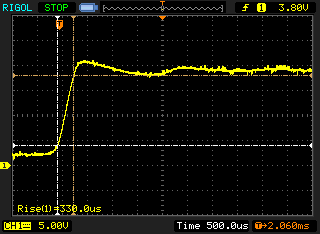
\includegraphics[width=\textwidth,height=0.4\textheight,keepaspectratio]{rise-time}
	\caption{Tiempo de subida de 2V a 20V de 330$\mu s$}
\end{figure}

\begin{figure}[H]
	\centering
	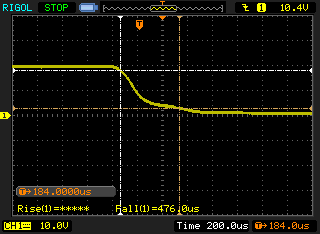
\includegraphics[width=\textwidth,height=0.4\textheight,keepaspectratio]{fall-time}
	\caption{Tiempo de bajada de 20V a 2V de $610\mu s$}
\end{figure}

\chapter{Conclusión}

El sistema es estable y funciona perfectamente con los parámetros del PID calculados en MATLAB tal como lo indicaba el modelo en la teoría. El ripple es ligeramente superior al calculado debido probablemente al ESR de los capacitores. La regulación de carga y de línea es excelente manteniendo la tensión prácticamente sin variación.

Algunas mejores posibles son el reemplazo del transformador de 50Hz por una fuente conmutada para poder sacar más potencia (la cual se encuentra limitada actualmente por el transformador) y reducir el peso. 

La utilización de un ADC de mayor resolución es también otra posible mejora que podría mejorar la regulación de carga ya que la variación actual es tan pequeña que no se encuentra dentro del rango detectable del ADC (que como se vio en la sección \ref{acondicionamiento-tensiones} es de 45mV).

\newpage
\chapter{Bibliografía y Contacto}

\begin{itemize}
	\item dsPIC33FJ16GS402 Datasheet - \url{http://ww1.microchip.com/downloads/en/DeviceDoc/70000318g.pdf}
	\item Marty Brown. (2001). Power Supply Cookbook 2nd Edition. USA: Newnes.
	\item Keith H. Billings. (1989). Switchmode Power Supply Handbook. USA: McGraw-Hill.
	\item Abraham I. Pressman. (2009). Switching Power Supply Design, Third Edition. USA: McGraw-Hill.
	\item Microchip WebSeminar - \url{http://www.microchip.com/stellent/groups/SiteComm_sg/documents/Training_Tutorials/en528035.pdf}
	\item Typical gate drive waveforms - \url{http://www.richieburnett.co.uk/temp/gdt/gdt2.html########.html}
	\item A Current Sensing Tutorial - Part II: Devices - \url{http://www.eetimes.com/document.asp?doc_id=1279415}
	\item SMPS AC/DC Reference Design User's Guide - \url{http://ww1.microchip.com/downloads/en/DeviceDoc/dsPICSMPS\%20AC_DC\%20Users\%20Guide.pdf}
	\item Amidon Iron Powder Toroidal Cores - \url{http://www.qrz.lt/ly1gp/amidon.html}
	\item Iron Powder Toroids - \url{http://www.catzco.com/toroids.htm}
	\item TI - Input and Output Capacitor Selection - \url{http://www.ti.com/lit/an/slta055/slta055.pdf}
	\item TI - Basic Calculation of a Buck Converter's Power Stage - \url{http://www.ti.com/lit/an/slva477b/slva477b.pdf}
	\item TI - Understanding Buck Power Stages in Switchmode Power Supply - \url{http://www.ti.com/lit/an/slva057/slva057.pdf}
	\item Linear Devices - Modeling and Loop Compensation Design of
	Switching Mode Power Supplies - \url{http://cds.linear.com/docs/en/application-note/AN149fa.pdf}
	\item Modeling of PID controller based SMPS using
	FPGA - \url{https://www.ijirset.com/upload/december/5-Modeling\%20of\%20PID\%20controller.pdf}
	\item Mathworks - Design a PID Controller Using Simulated I/O Data - \url{https://www.mathworks.com/help/slcontrol/examples/design-a-pid-controller-using-simulated-i-o-data.html}
	\item Mathworks - Plotting System Responses - \url{https://www.mathworks.com/help/control/examples/plotting-system-responses.html}
	\item Toroids Info - \url{http://toroids.info/}
	\item Foro diyAudio - \url{www.diyaudio.com}
	\item Foro diySMPS - \url{www.diysmps.com}
	\item Sitio Q\&A - Electronics StackExchange - \url{http://electronics.stackexchange.com/}
\end{itemize}

Para cualquier duda o mayor información pueden escribirnos a \href{mailto:torti.max@gmail.com}{torti.max@gmail.com} (Torti Andrés) o \href{mailto:anchinoleonardo@gmail.com}{anchinoleonardo@gmail.com} (Anchino Leonardo).

\end{document}